% Use the custom `CustomDocument` class
% - A4 paper size
% - 12pt base font size
% - Fourier as the main typeface
% - One-sided document setup
% - Custom bibliography setup to use BibLaTeX
\documentclass[a4paper,12pt,fourier,oneside,custombib]{Classes/CustomDocument}

% ******************************************************************************
% ****************************** Custom Margin *********************************

% Add `custommargin' in the document class options to use this section
% Set {innerside margin / outerside margin / topmargin / bottom margin}  and
% other page dimensions

% Add spaces between paragraphs
%\setlength{\parskip}{0.5em}
% Ragged bottom avoids extra whitespaces between paragraphs
\raggedbottom
% To remove the excess top spacing for enumeration, list and description
%\usepackage{enumitem}
%\setlist[enumerate,itemize,description]{topsep=0em}

% ***************************** Header Formatting ******************************
% Custom Header with Chapter Number, Page Number and Section Numbering

\usepackage{fancyhdr} % Define custom header
\pagestyle{fancy}
\fancyhf{}
\rhead{\leftmark}
\cfoot{\thepage}

% *****************************************************************************
% ******************* Fonts (like different typewriter fonts etc.)*************

% Add `customfont' in the document class option to use this section

\ifsetCustomFont
  % Set your custom font here and use `customfont' in options. Leave empty to
  % load computer modern font (default LaTeX font).
  %\RequirePackage{helvet}

  % For use with XeLaTeX
  %  \setmainfont[
  %    Path              = ./libertine/opentype/,
  %    Extension         = .otf,
  %    UprightFont = LinLibertine_R,
  %    BoldFont = LinLibertine_RZ, % Linux Libertine O Regular Semibold
  %    ItalicFont = LinLibertine_RI,
  %    BoldItalicFont = LinLibertine_RZI, % Linux Libertine O Regular Semibold Italic
  %  ]
  %  {libertine}
  %  % load font from system font
  %  \newfontfamily\libertinesystemfont{Linux Libertine O}
\fi

% *****************************************************************************
% **************************** Custom Packages ********************************

% ************************* Algorithms and Pseudocode **************************

%\usepackage{algpseudocode}


% ********************Captions and Hyperreferencing / URL **********************

% Captions: This makes captions of figures use a boldfaced small font.
%\RequirePackage[small,bf]{caption}

\RequirePackage[labelsep=space,tableposition=top]{caption}
\renewcommand{\figurename}{Fig.} %to support older versions of captions.sty


% *************************** Graphics and figures *****************************

%\usepackage{rotating}
%\usepackage{wrapfig}

% Uncomment the following two lines to force Latex to place the figure.
% Use [H] when including graphics. Note 'H' instead of 'h'
%\usepackage{float}
%\restylefloat{figure}

% Subcaption package is also available in the sty folder you can use that by
% uncommenting the following line
% This is for people stuck with older versions of texlive
%\usepackage{sty/caption/subcaption}
\usepackage{subcaption}

% ********************************** Tables ************************************
\usepackage{booktabs} % For professional looking tables
\usepackage{multirow}

%\usepackage{multicol}
%\usepackage{longtable}
%\usepackage{tabularx}


% *********************************** SI Units *********************************
\usepackage{siunitx} % use this package module for SI units


% ******************************* Line Spacing *********************************

% Choose linespacing as appropriate. Default is one-half line spacing as per the
% University guidelines

% \doublespacing
% \onehalfspacing
% \singlespacing


% ************************ Formatting / Footnote *******************************

% Don't break enumeration (etc.) across pages in an ugly manner (default 10000)
%\clubpenalty=500
%\widowpenalty=500

%\usepackage[perpage]{footmisc} %Range of footnote options


% *****************************************************************************
% *************************** Bibliography  and References ********************

%\usepackage{cleveref} %Referencing without need to explicitly state fig /table

% Add `custombib' in the document class option to use this section
\ifuseCustomBib
 %  \RequirePackage[round, sort, numbers, authoryear]{natbib} % CustomBib

%\bibliographystyle{apalike}

% If you would like to use biblatex for your reference management, as opposed to the default `natbibpackage` pass the option `custombib` in the document class. Comment out the previous line to make sure you don't load the natbib package. Uncomment the following lines and specify the location of references.bib file

\RequirePackage[
 backend=biber,
 style=apa,
 sorting=nty,
 natbib=true,
 url=true,
 doi=true]{biblatex}
\bibliography{References/references} %Location of references.bib only for biblatex

\fi


% ******************************************************************************
% ************************* User Defined Commands ******************************
% ******************************************************************************

% *********** To change the name of Table of Contents / LOF and LOT ************

%\renewcommand{\contentsname}{My Table of Contents}
%\renewcommand{\listfigurename}{My List of Figures}
%\renewcommand{\listtablename}{My List of Tables}


% ********************** TOC depth and numbering depth *************************

\setcounter{secnumdepth}{2}
\setcounter{tocdepth}{2}


% ******************************* Nomenclature *********************************

% To change the name of the Nomenclature section, uncomment the following line

%\renewcommand{\nomname}{Symbols}


% ********************************* Appendix ***********************************

% The default value of both \appendixtocname and \appendixpagename is `Appendices'. These names can all be changed via:

%\renewcommand{\appendixtocname}{List of appendices}
%\renewcommand{\appendixname}{Appndx}

% *********************** Configure Draft Mode **********************************

% Uncomment to disable figures in `draft'
%\setkeys{Gin}{draft=true}  % set draft to false to enable figures in `draft'

% These options are active only during the draft mode
% Default text is "Draft"
%\SetDraftText{DRAFT}

% Default Watermark location is top. Location (top/bottom)
%\SetDraftWMPosition{bottom}

% Draft Version - default is v1.0
%\SetDraftVersion{v1.1}

% Draft Text grayscale value (should be between 0-black and 1-white)
% Default value is 0.75
%\SetDraftGrayScale{0.8}


% ******************************** Todo Notes **********************************
%% Uncomment the following lines to have todonotes.

%\ifsetDraft
%	\usepackage[colorinlistoftodos]{todonotes}
%	\newcommand{\mynote}[1]{\todo[author=kks32,size=\small,inline,color=green!40]{#1}}
%\else
%	\newcommand{\mynote}[1]{}
%	\newcommand{\listoftodos}{}
%\fi

% Example todo: \mynote{Hey! I have a note}

% Fix header height
\usepackage{titlesec}
\titleformat{\chapter}[display]
{\normalfont\huge\bfseries}{\chaptertitlename\ \thechapter}{20pt}{\Huge}   
\titlespacing*{\chapter}{0pt}{-20pt}{40pt}

\title{Enabling General Applicability for Brain-Computer Interface Software Through Cloud Computing}
\author{Daniel Burger}
\dept{Department of Web Development}
\university{Middlesex University London}

% Crest minimum should be 30mm
\crest{
\includegraphics[width=0.2\textwidth]{middlesex-university.pdf}}

%% Submission text
\renewcommand{\submissiontext}{This thesis is submitted for the degree of}
\degreetitle{Bachelor of Science, Web Development}
\college{SAE Institute Zürich}

% Meta information
\subject{Bachelor Thesis}
\keywords{
  In-Ear EEG,
  EEG,
  IDUN Technologies,
  Electroencephalography,
  Virtual Reality,
  Web Application,
  Cloud Computing,
  Human-Computer Interaction,
  Software Engineering,
  Web Development,
  Brain/Cloud Interface,
  Neural/Cloud Interface
  Brain-Machine Interface,
  Brain-Computer Interface,
}


\pagenumbering{roman} % Start with lowercase Roman numbers
\setcounter{page}{1}
\begin{document}

\frontmatter
\maketitle
\begin{abstract}
	Saepe veniam laudantium qui sint odio doloribus ea itaque. Et aliquid deserunt animi. Voluptas id expedita qui reiciendis placeat debitis praesentium autem. Qui quia voluptatibus alias recusandae at velit tenetur velit. Aperiam aliquid possimus fugiat autem in. Quibusdam libero voluptatem sit. In est est voluptas. Eum et molestiae repudiandae totam. Doloremque aut quae fugiat quia rerum sed. Commodi ad repudiandae sed laborum odio. Saepe veniam laudantium qui sint odio doloribus ea itaque. Et aliquid deserunt animi. Voluptas id expedita qui reiciendis placeat debitis praesentium autem. Qui quia voluptatibus alias recusandae at velit tenetur velit. Aperiam aliquid possimus fugiat autem in. Quibusdam libero voluptatem sit. In est est voluptas. Eum et molestiae repudiandae totam. Doloremque aut quae fugiat quia rerum sed. Commodi ad repudiandae sed laborum odio.
\end{abstract}
\begin{dedication}

  This work is dedicated to the IDUN Technologies\footnote{Neurotechnology startup in Zürich: https://iduntechnologies.com} team, who have been extremely helpful in my journey into the neurotechnology industry. They taught me a lot about working in a scientific setting and allowed me to investigate various aspects of non-invasive brain-computer interfaces in conjunction with cloud computing and virtual reality.

  \hfill \break

  I'd also like to thank the open-source collective Poimandres\footnote{Developers behind various Three.js-related libraries: https://docs.pmnd.rs} for their WebGL libraries, which have helped me understand some of the most difficult challenges in 3D graphics programming which was a fundamental part of the practical part of my bachelor project.

\end{dedication}

\tableofcontents
\thispagestyle{empty}
\cleardoublepage
\pagenumbering{Roman} % Continue with uppercase Roman numbers
\setcounter{page}{1}
\listoffigures
\listoftables
\printnomenclature

\mainmatter
\pagenumbering{arabic}
\setcounter{page}{1}

\chapter{Introduction}
\graphicspath{{Chapter1/Figs/}{Chapter1/Figs/}}

\section{Background}
\label{chapter1-background}

There has been a long-standing interest in developing neural interfaces, systems that sense electrical impulses from the nervous system and use them to intercommunicate with the human brain. Successful research into the development of technologies that enable neural interfaces has been going on for decades \citep{vidal_real-time_1977}. Progress has accelerated significantly in the past few years, especially since the advent of modern processing capabilities such as in deep learning with convolutional neural networks (CNN) or generative adversarial networks (GAN) \citep{gonfalonieri_deep_2019}. In particular, a related discipline called brain-computer interfacing (BCI), a field focused on the direct interaction between brains and computers, has accumulated much momentum since the popularity of companies like Neuralink and Kernel.

One aspect of neural interfaces is hardware tailored to the human body. Whether it is an invasive sensor, such as in electrocorticography (ECoG), a method which uses electrodes placed on the surface of the brain, or a non-invasively placed sensor on the body, such as in electroencephalography (EEG). Both methods measure electrical activities produced by neurons; however, with decreasing spatial precision, the farther the electrode is placed from the brain, the more body structures (e.g. bones) are between firing neurons and the measuring sensor. The other aspect is software that reads and interprets data of these hardware sensors. Both aspects present their own set of challenges and complexities. Nonetheless, complete and applicable neural interfaces work in practice and have been used for many years in patients with neurological disorders \citep{braingate_publications_nodate}. There are also consumer and non-clinical neural interfaces available, such as the Neurosity and OpenBCI products, which aim to democratise the use of EEG sensors by offering low-cost hardware and simple-to-use software.

This thesis will focus on the software aspect of non-invasive neural interfaces and the challenges and complexities that arise in the given context of modern software engineering for production-ready end-user facing brain-computer interface applications.

\nomenclature[cnn]{CNN}{Convolutional neural networks}
\nomenclature[gan]{GAN}{Generative adversarial networks}
\nomenclature[bci]{BCI}{Brain-computer interface}
\nomenclature[ecog]{ECoG}{Electrocorticography}
\nomenclature[eeg]{EEG}{Electroencephalography}

% Kreative Darstellung der kreativen Idee und Zieldefinition. Wichtig ist hier, dass zwar eine klare Zielvorstellung (Umfang, Pflichtenheft mit Teilzielen, welche Qualität soll erreicht werden) vorhanden ist, aber der genaue Weg noch nicht exakt feststeht. Möglicher Umfang: 10 Prozent der Gesamtlänge.

\section{Project motivation}
\label{chapter1-project-motivation}

The possibilities of connecting the human brain with computers are almost limitless because one has to imagine that we are the brain, that our own perception of the world, all our feelings, thoughts and actions are supposed to be contained in the electrical impulses of our brain. The ability to communicate directly with our thoughts and the outside world — whether through digital or physical objects — is a fantastic prospect. There are several use cases: Controlling prosthetic limbs for amputees, communication for people with locked-in syndrome, diagnosing neurological problems and improving the mental capacities of elderly patients are promising examples, to name a few.

\begin{figure}
  \centering
  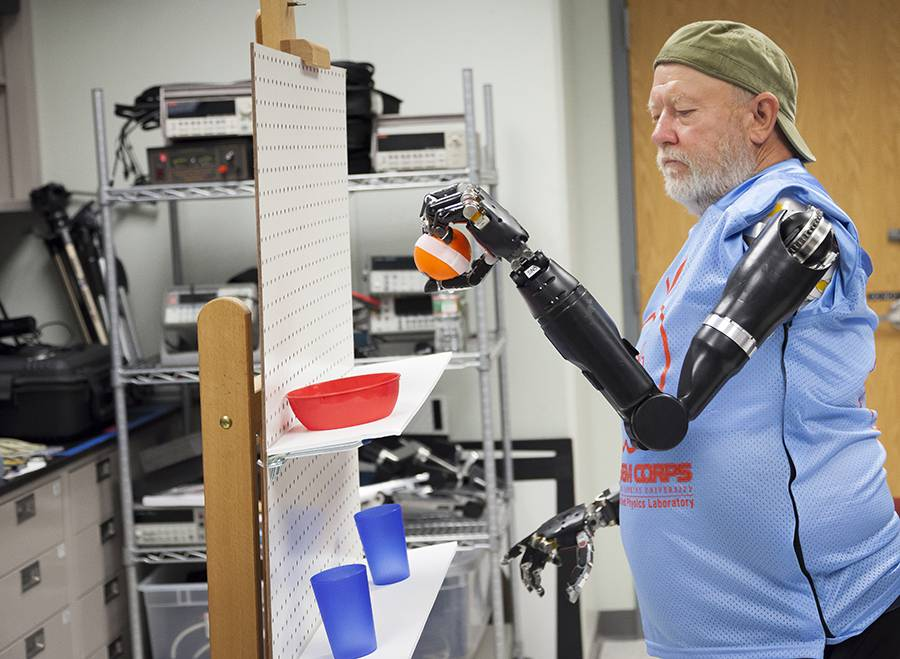
\includegraphics[width=\linewidth]{prostetic-arms.jpg}
  \captionsetup{justification=centering,width=0.9\textwidth}
  \caption{Les Baugh, an amputee, is using a neural interface to control two robotic arms.}
  \label{fig:prostetic-arms}
\end{figure}

It may appear evident that neural interfaces can significantly impact the field of therapeutics and accessibility for a small subset of the human population. However, one can envision not only alleviating deplorable living conditions but also improving the lives of healthy people through more natural or efficient ways of interacting or by directly altering human brains themselves. Because most current neural interface applications concentrate on the first aspect of therapeutics and accessibility, other use cases, such as stimulating the brain to improve concentration, modifying cognitive load, or even uploading new knowledge directly into the brain, may appear to be science fiction ideas.

Regardless, many intelligent people — research labs or even entire companies — are developing neural interface hardware and software aimed at the general population without conditions that envision a future for such use cases in the long term. The applicability of a neural interface system to the mainstream depends on several factors, presumably an important factor of which is the hardware's form factor.

% Goal: Give an overview of the relevant scientific literature.
% What is known? Which questions remain open? Are there conflicts in the literature?
% - Several studies have shown that…
% - While some studies suggested that X (References) other studies pointed in the opposite
% direction (References)
% - The findings of some studies suggested that X (References). In contrast, other studies have shown that Y (References)
% - Two theories have been proposed to explain this phenomenon. According to theory X….
% - Three lines of research are relevant to this question. First,…
% - Devin et al. (2003) were one of the first who found evidence that…
% - Overall, it has remained unclear whether…
% - Taken together, it remains an open question whether…

\section{Research question}
\label{chapter1-research-question}

% Goal 1: State your research question
% - The goal of the present article is to…
% - The research question of the present article is…
% Goal 2: State your hypotheses/ predictions
% - We hypothesize that…
% - We predict that…
% - Two hypotheses are conceivable…
% - Our primary hypothesis is that…
% - Drawing on theory X, we hypothesize that…
% Goal 3: Give a rough outline of your research
% - We tested whether patients with a diagnosed major depression would report less depressive
% feelings after treatment X compared to a placebo treatment.
% - To test this hypothesis, we ….
% - To answer this question, we …
% - For this purpose, we conducted three studies. First,… Second,… Third,…
% - To shed more light on this, we used a combination of computer simulations and empirical
% studies. First, we used computer simulations to determine what behaviour would arise if theory
% 3
% X is true and what behaviour would arise if theory Y was true. Next, we tested these two
% predictions in three empirical studies.
% - The present article consists of three sections. In section 1, … In section 2,… In section 3

\section{Goals}
\label{chapter1-goals}

% o Does your introduction go from broad (topic) to specific (your research)?
% o Did you make clear why your topic is important?
% o Did you describe just enough research so that readers can understand how your
% research is the next logical step?
% o Did you make clear how your research is novel?
% o Did you make clear what is speculation, and what are established facts?
% o Did you add citations for everything you present as facts?
% o Did you use common scientific jargon?
% o Did you explain the jargon you use? % Introduction
\chapter{Research Context}
\graphicspath{{Chapter2/Figs/}{Chapter2/Figs/}}

This chapter describes the research question's context and the current literature findings. The reader is educated on neuroscientific limitations, the state of current non-invasive and unidirectional BCIs, the paradigm shift in developing cloud-based and production-ready software and the requirement-based definition of a N/CI.

\section{Limitations of BCIs}
\label{chapter2-limitations-of-bcis}

The possibilities of BCIs are not without limitations. In addition to the hardware limitations, the author addresses a broader issue related to neuropsychology that directly correlates with the software aspects, in addition to the challenges of computability.

\subsection{Decoding brain data}
\label{chapter2-decoding-brain-data}

As outlined in the previous chapter, a holistic view of BCI must take into account the aspect of decoding measured neural data and making it intelligible to computer software. It is important to emphasise that the task of decoding neural data is different from decoding thoughts, which is a critical factor for software. Moreover, decoding neural data and extracting the thoughts behind it so that the software can understand them are disciplines on their own. For example, getting computers to recognise letters written on a photograph is a very different problem from reading the written words in the sentences (i.e. computer vision and natural language processing).

Another part is understanding the sentences and their meaning, as in natural language understanding (NLU). NLU is considered an AI-hard problem, which means that the difficulty of these computational problems is equivalent to solving the central problem of artificial general intelligence\footnote{Based on the assumption that general human-level intelligence is computable.} (AGI) \citep{demasi_theoretical_2010}. Understanding less structured data, such as EEG data, is more complicated than understanding structured and human-generated syntax such as written language because it contains more hidden features than a paragraph of text. As a result, the author assumes that understanding brain data might be considered an AI-hard problem.

\subsection{Abstract thoughts}
\label{chapter2-abstract-thoughts}

\begin{figure}[ht]
  \centering
  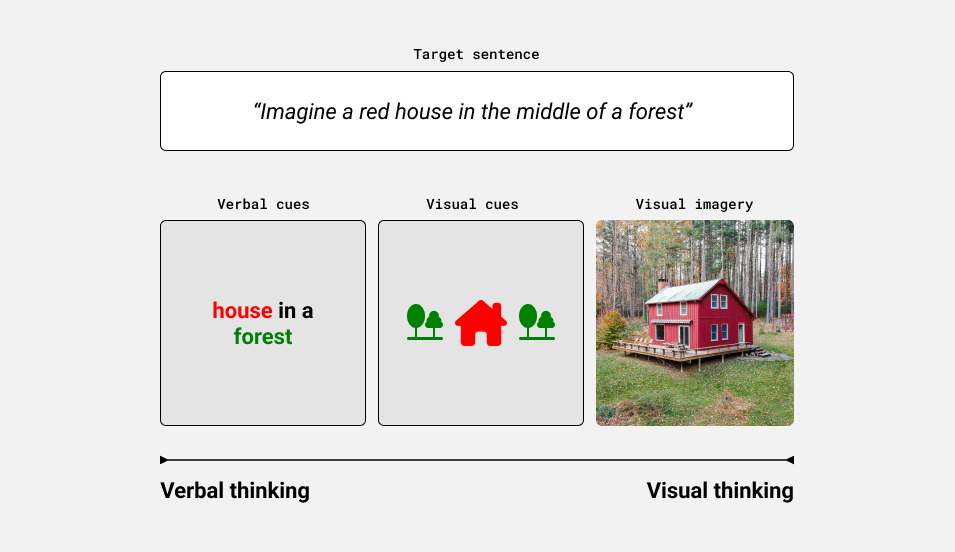
\includegraphics[width=\linewidth]{visual-thinking.png}
  \caption{Difference between verbal and visual thinking using the target sentence of a red house in the middle of a forest (own representation, 2022).}
  \label{fig:visual-thinking}
\end{figure}

To further emphasise the complexity of interpreting neural data, a practical example will be presented: Imagine a red house in the middle of a forest. Depending on the individual thought process, one might imagine the house with temporary visual imagery in mind, as in visual thinking, or one might imagine it more verbally, such as conceptually comprehending each word sequentially of what a red house is and that it is located in a forest \citep{amit_asymmetrical_2017}. Additionally, it should also be addressed that different types of thoughts exist at different levels of abstraction and complexity. One can assume that the visual image of a red house in the forest is more abstract and far-fetched than, say, the movement of one's own thumbs, which has a clear physical counterpart. It gets even more complicated when one imagines concepts that are inconceivable to visualise, such as the idea of a company. A company is only an abstract, collectively agreed upon concept without a physical counterpart\footnote{Some people might think of a company building when imaging a company, others might imagine their website, their logo or physical products} and is, therefore, even less straightforward and more complex to decode the meaning of measured brain activity than the other mentioned examples of the red house.

\subsection{Technological limitations}
\label{chapter2-technological-limitations}

\begin{figure}[ht]
  \centering
  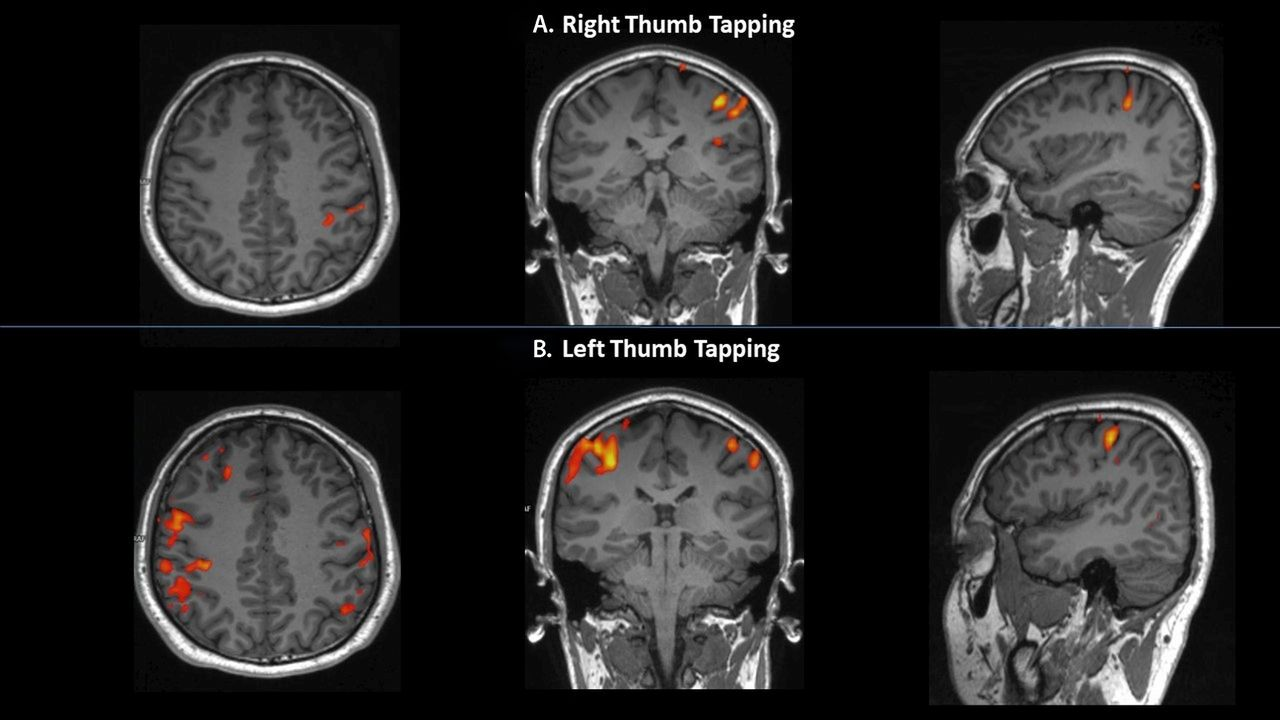
\includegraphics[width=\linewidth]{fmri-scan.jpg}
  \caption{Image of localised activation of neurons during right and left thumb movement using functional magnetic resonance imaging (fMRI) \citep{rashid_bilateral_2018}.}
  \label{fig:fmri-scan}
\end{figure}

Most functional tasks of the brain are localised, which means that these signals are generated by local brain areas that can be identified, such as the motor cortex, which has been shown to be responsible for muscle movement as shown in \autoref{fig:fmri-scan} \citep{rashid_bilateral_2018}. Examining the areas of the brain responsible for activating individual muscle strands can yield a comparable response of muscle stimulation in the brain and thus be measured as output for software to move a prosthesis, for example. However, the more specific, less functional, more behavioural and abstract the thoughts are, the less the brain areas are spatially visible. The intent of identifying, for example, the thought of a red house in a forest in verbal thought, the author identified three technological problem statements:

\begin{itemize}
  \item To understand single thoughts, it is essential to have sufficiently clear data from experiments with a certain level of detail (e.g., at the level of detail related to the firing of action potentials of individual neurons) as well as temporal precision (an action potential takes about 1 ms to arise) to perform studies to extract possible localisation of individual thoughts. Current neuroimaging technologies cannot capture every process in sufficient detail of the entire brain at once to extract the activity of, e.g. individual neurons while also having high temporal precision.
  \item Even if we could measure every single neuron in the brain with high temporal precision, we would have an extreme amount of data generated concisely. Let us say we would collect a float per neuron that represents the rate of change in voltage with respect to time with a frequency of 1 ms and then record each neuron in the brain a million times a second, taking into account that the average human brain has around 86 billion neurons; we would generate 305.53337637684 petabytes of data per second. This is currently not feasible for commercially available storage and processing resources.
  \item Even if we have the technology, it is a challenge because reproducibility of experiments is very difficult for neuroscientific studies. It is probably impossible to generate clean-slate neural data that is comparable to previously recorded data. Our neurophysiological brain structure changes over time due to neuroplasticity \citep{puderbaugh_neuroplasticity_2022}, and we are in different states of mind every millisecond of our existence, which can have different influences, such as insufficient sleep, something disturbing someone, mental distraction due to an important event that may have occurred since the last measurement, or a salient thought that occurs during a measurement.
\end{itemize}

\subsection{Lack of data}
\label{chapter2-lack-of-data}

As pointed out in the previous section, points 2 and 3 depend on advances in data storage systems or the possibility that we do not actually need such precise brain data to understand single thoughts. However, to address point 1, some promising solutions already exist for measuring large parts of the brain with high temporal and spatial precision, such as time-domain functional near-infrared spectroscopy (TD-fNIRS), which Kernel employs in its Kernel Flow device \citep{ban_kernel_2021}. The TD-fNIRS system detects changes in concentrations of oxygenated (oxyHb) and deoxygenated brain cell activity by using near-infrared light in response to neuronal activity. This is a newer and more promising technology for measuring the full spectrum of neuroimaging of brain activity when compared to, e.g. EEG. According to Kernel, the precision of TD-fNIRS is sufficient for better understanding the brain and using it for BCI applications. They, however, claim that collecting and organising longitudinal brain data from a variety of subjects is the key to solving the most difficult challenges in neuroscience \citep{kernel_hello-humanitypdf_nodate}.

Based on Kernel's claim, a recent publication from 2022 also claims that even data sets with several hundred people are too tiny to consistently offer insights about the brain \citep{marek_reproducible_2022}. As a result, most published neuroscience studies with dozens or even hundreds of people could all be incorrect. In such research, brain structure and activity variations have been linked to variances in cognitive capacity, mental health, and other behavioural features. Numerous studies, for example, have revealed brain structure or activity patterns that may help distinguish persons with depression from those who are not. Neuromarkers of behavioural features are frequently sought in studies. The recent publication from \citeauthor{marek_reproducible_2022} claims that most of these so-called neuro markers would not work when the collected data set is more extensive, which prose a general problem for the field of neuroscience.

This is both fascinating and a significant constraint for BCIs, because understanding the brain is essential to making sense of the measured and classified data for interfacing with it. Therefore a large amount of brain data collected in reproducible experiments is a must for production-ready and mainstream-ready BCIs. UK Biobank's collection of brain scans is one of the first efforts to solve this problem \citep{noauthor_imaging_nodate}, but it is still far from what we might need. Marek himself claims that we might even need millions of data sets to start understanding the brain \citep{callaway_can_2022}. This is where customer-oriented BCIs could come into play because the adoption rate of a device capable of being used in everyday life is higher than that of experimental subjects, making it more likely to generate larger and longitudinal data sets. We will further discuss this in a later chapter.

\section{BCI landscape}
\label{chapter2-research-landscape}

In this section, we will discuss the current state of real-life and non-invasive BCIs, their applications and the distinctions that lie within their software offerings.

\subsection{Real-world BCI applications}
\label{chapter2-real-world-bci-applications}

As mentioned in \autoref{chapter1-background}, consumer-oriented BCI products are already commercially available. Based on Google Trends\footnote{Google Trends: https://trends.google.com} the products from OpenBCI are most likely the most popular. OpenBCI does not provide a specific use case but rather a hardware and software stack that is universally applicable. It can be used in research where EEG is to be used or in developing BCI applications. Several neurofeedback or research apps have been created using OpenBCI's products \citep{openbci_openbci_nodate}. Taking this information into consideration, we can see that the OpenBCI customer is responsible for developing their own BCI application or incorporating it into their research, rather than having a sophisticated end-user application from OpenBCI.

Another example is NextMind, which was recently acquired by Snapchat \citep{heater_snap_2022}. They do not have an end-user application for their BCI\footnote{NextMind and OpenBCI have both a graphical user interface (GUI) application for the control and quality check of their hardware, but neither is intended for end-users.}, but they do offer an SDK for the Unity real-time engine to use their technology for brain-controlled actions in video games. One significant difference between NextMind and OpenBCI is that NextMind includes a built-in classification of brain waves captured by hardware, in this case, classification of active visual focus on virtual objects based on steady-state visual evoked potentials (SSVEP). Because their business model was presumably based on the unique selling point of their active visual focus classifier, NextMind did not provide access to the raw EEG data collected by the sensors. Nonetheless, NextMind's product is less focused on a specific use case, as its applicability is limited to game developers.

\begin{figure}[!htb]
  \minipage{0.32\textwidth}
  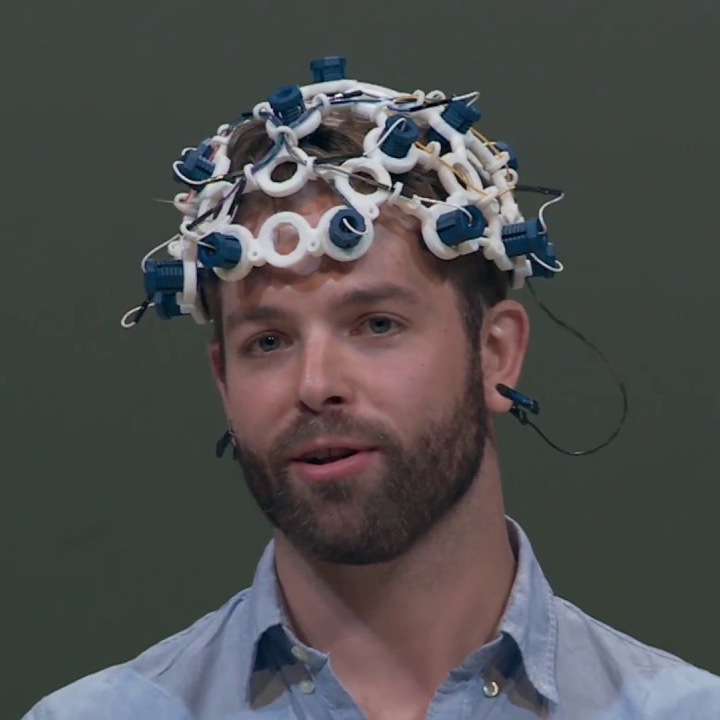
\includegraphics[width=\linewidth]{openbci.jpeg}
  \caption{OpenBCI's EEG \\ device \citep{be_superhvman_conor_2017}}
  \label{fig:openbci}
  \endminipage\hfill
  \minipage{0.32\textwidth}
  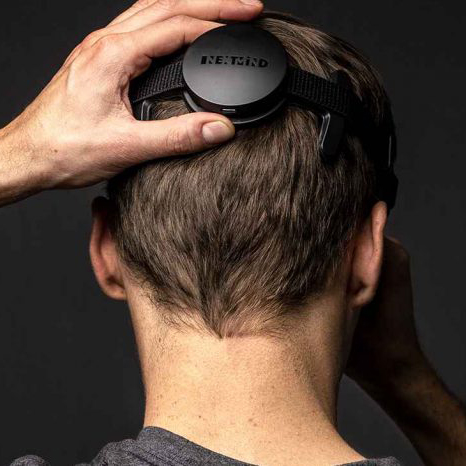
\includegraphics[width=\linewidth]{nextmind.jpeg}
  \caption{NextMind's BCI \\ device \citep{louise_neurotechnology_2019}}
  \label{fig:nextmind}
  \endminipage\hfill
  \minipage{0.32\textwidth}%
  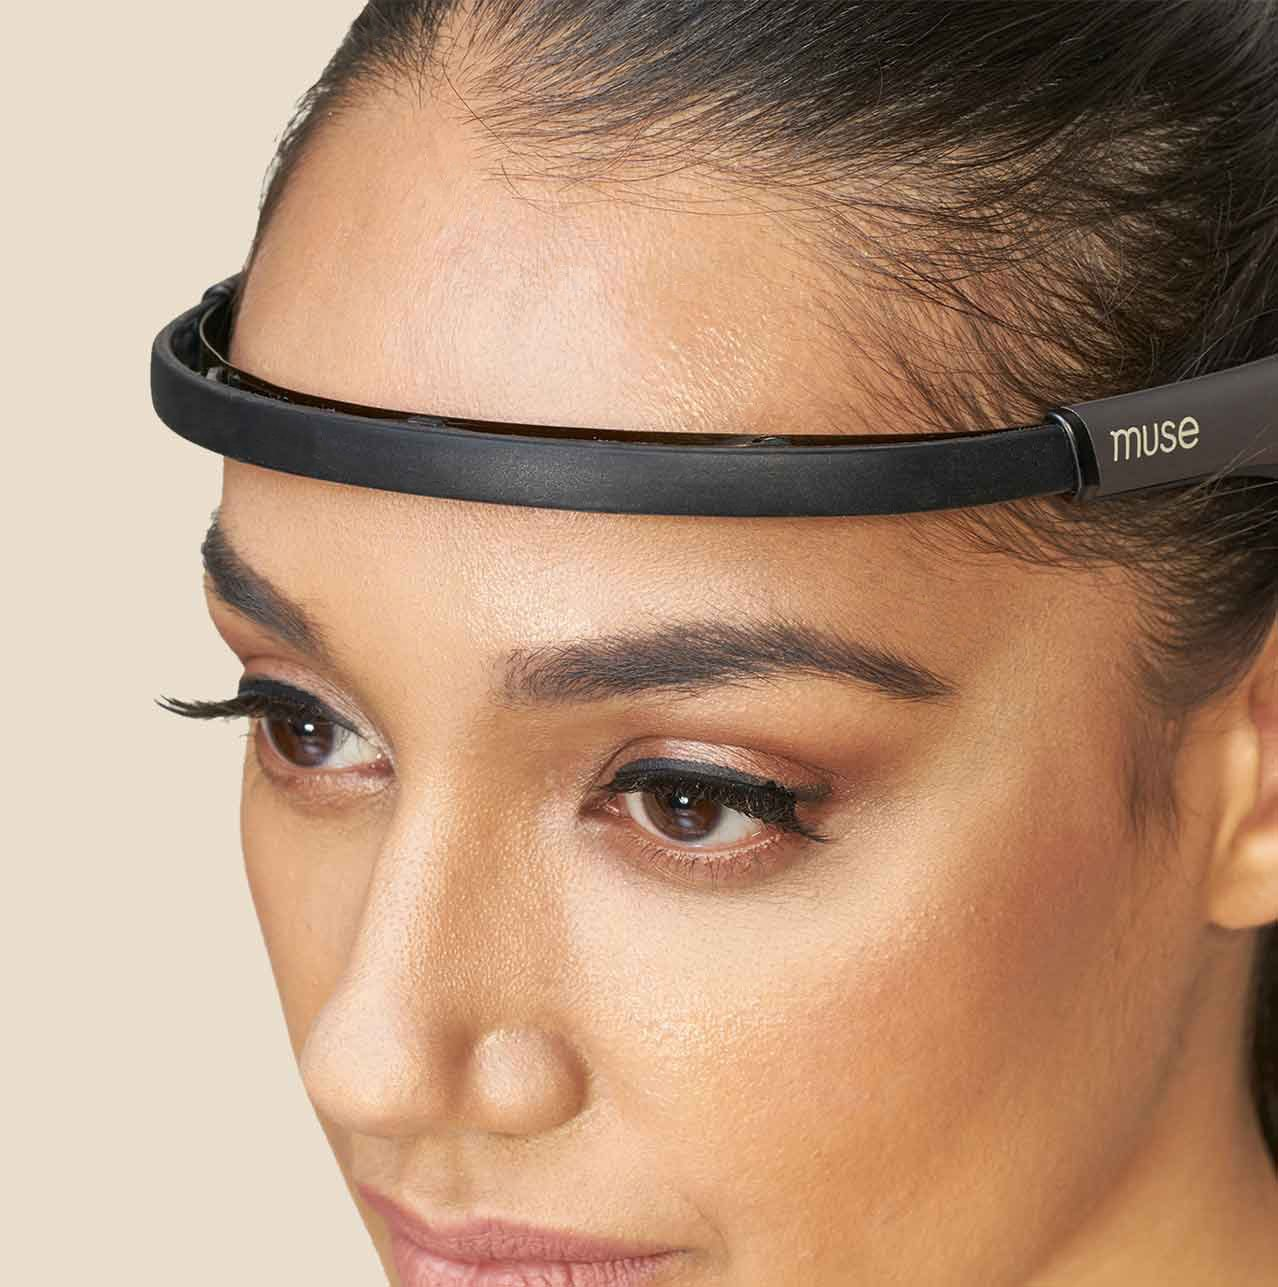
\includegraphics[width=\linewidth]{muse.jpeg}
  \caption{Muse's meditation \\ headband \citep{muse_muse_nodate}}
  \label{fig:muse}
  \endminipage
\end{figure}

A relatively closed and specific BCI is, for example, the EEG headband by Muse. Its purpose is to measure meditation and sleep. They also offer an end-user app to help people better understand their meditation and sleep and how to improve them. The Muse headband is not unidirectional BCI per se, as there is also biofeedback based on neural signals, but the vital difference between Muse and, e.g. OpenBCI is that they abstract away the neurotechnology. Users do not need to know anything about neuroscience, neurotechnology or the interpretation and classification of brain data to get useful functionality for their use case. They also do not need to understand the software system's underlying architecture. They only need to know how to pair the device with their smartphone via Bluetooth.

Aside from full-stack BCI solutions, where a company provides a complete BCI solution including hardware and software, some companies focus solely on the software aspect of neural data. Neuromore, a company based in Florida and Germany that provides a software platform for everything related to neural signal processing and BCI, is one example. The company is hardware agnostic, which means one can plug any hardware or sensor into their computer and connect it to the Neuromore Studio software. Neuromore Studio is free and open-source software that runs locally on various platforms, including Windows and macOS. It provides a variety of drag-and-drop interfaces for creating and managing signal processing pipelines, even including machine learning classifiers. For example, one can transform EEG data to extract band power, create triggers based on band power selection, and generate conditional outputs for a game to, e.g. move a character.

\begin{figure}[ht]
  \centering
  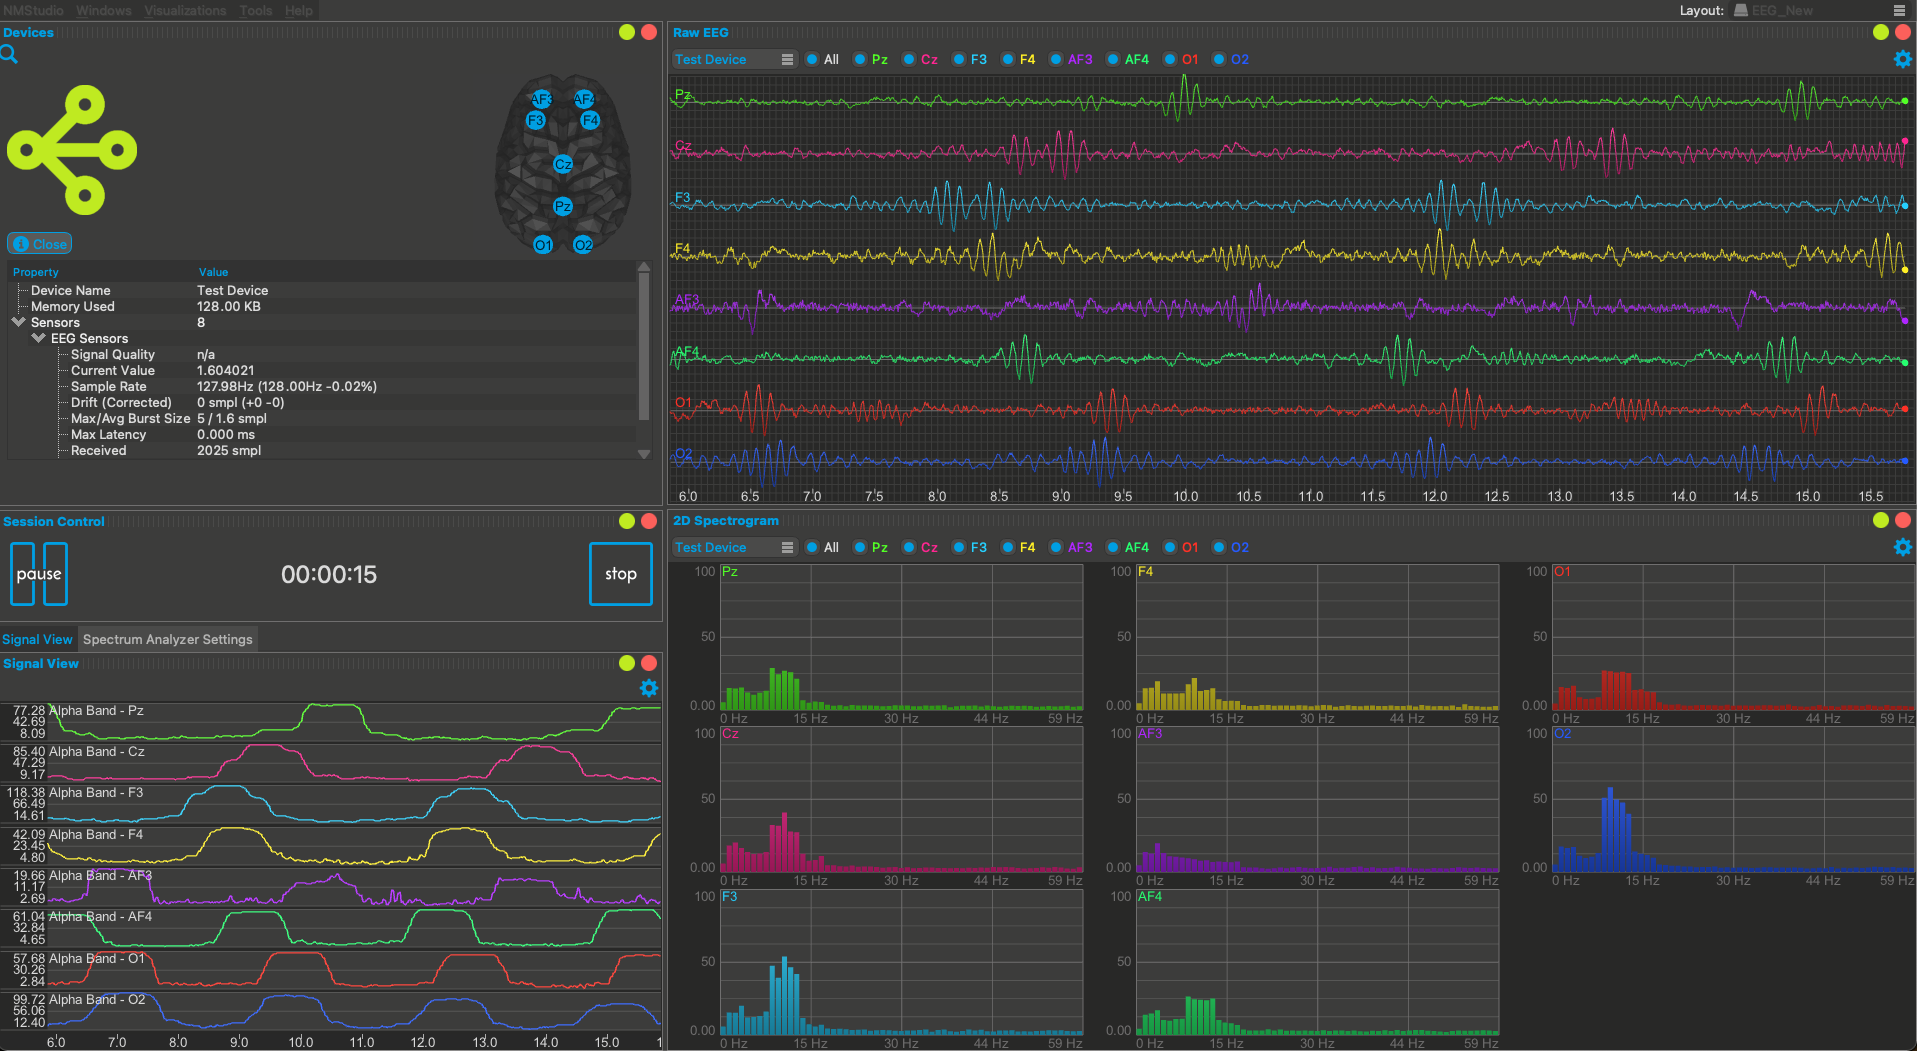
\includegraphics[width=\linewidth]{neuromore.png}
  \caption{Screenshot of the Neuromore Studio software \citep{neuromore_neuromore_nodate}.}
  \label{fig:neuromore}
\end{figure}

The author attempts to differentiate the offerings of the consumer-oriented BCIs mentioned: They either provide the hardware (with software that at least connects to the device) but are then more broadly applicable to use cases not defined by the company behind the BCI, such as OpenBCI, or they are application-specific in terms of both the software and the hardware, such as the Muse headband\footnote{Third-party developers have reverse-engineered the Bluetooth features to access Muse's raw EEG data and turn it into a general-purpose device.}.

Although this paper focuses on consumer-oriented BCIs, the applications of various BCI offerings can still be distinguished based on whether they are more consumer-oriented or research-oriented, such as the distinction between, e.g. NeuroSky\footnote{NeuroSky website: https://neurosky.com} for hobbyists and Emotiv's\footnote{Emotiv website: https://emotiv.com} EEG systems, which are more research-oriented.

However, NeuroSky and Emotiv provide a research version and a consumer or enterprise version of their software and hardware, aiming for general-purpose applicability across customer segments and use cases.

Other considerations include whether the applications are rather steady-state evoked, such as based on a frequency of noise laid on top of virtual objects to detect which object the person is looking at (e.g. as NextMind is doing), or whether they track the totality of mental states without evoking neural signals with external stimuli, such as in tracking sleep or concentration levels, both of which arise primarily evoked from inside the mind. This distinction can be made as passive, active or reactive BCI, as \citeauthor{alimardani_passive_2020} coined in their work on passive BCIs \citep{alimardani_passive_2020}. However, we do not want to include this dimension because it would introduce unnecessary and additional complexities related to the BCI software application layer.

\begin{figure}[!ht]
  \centering
  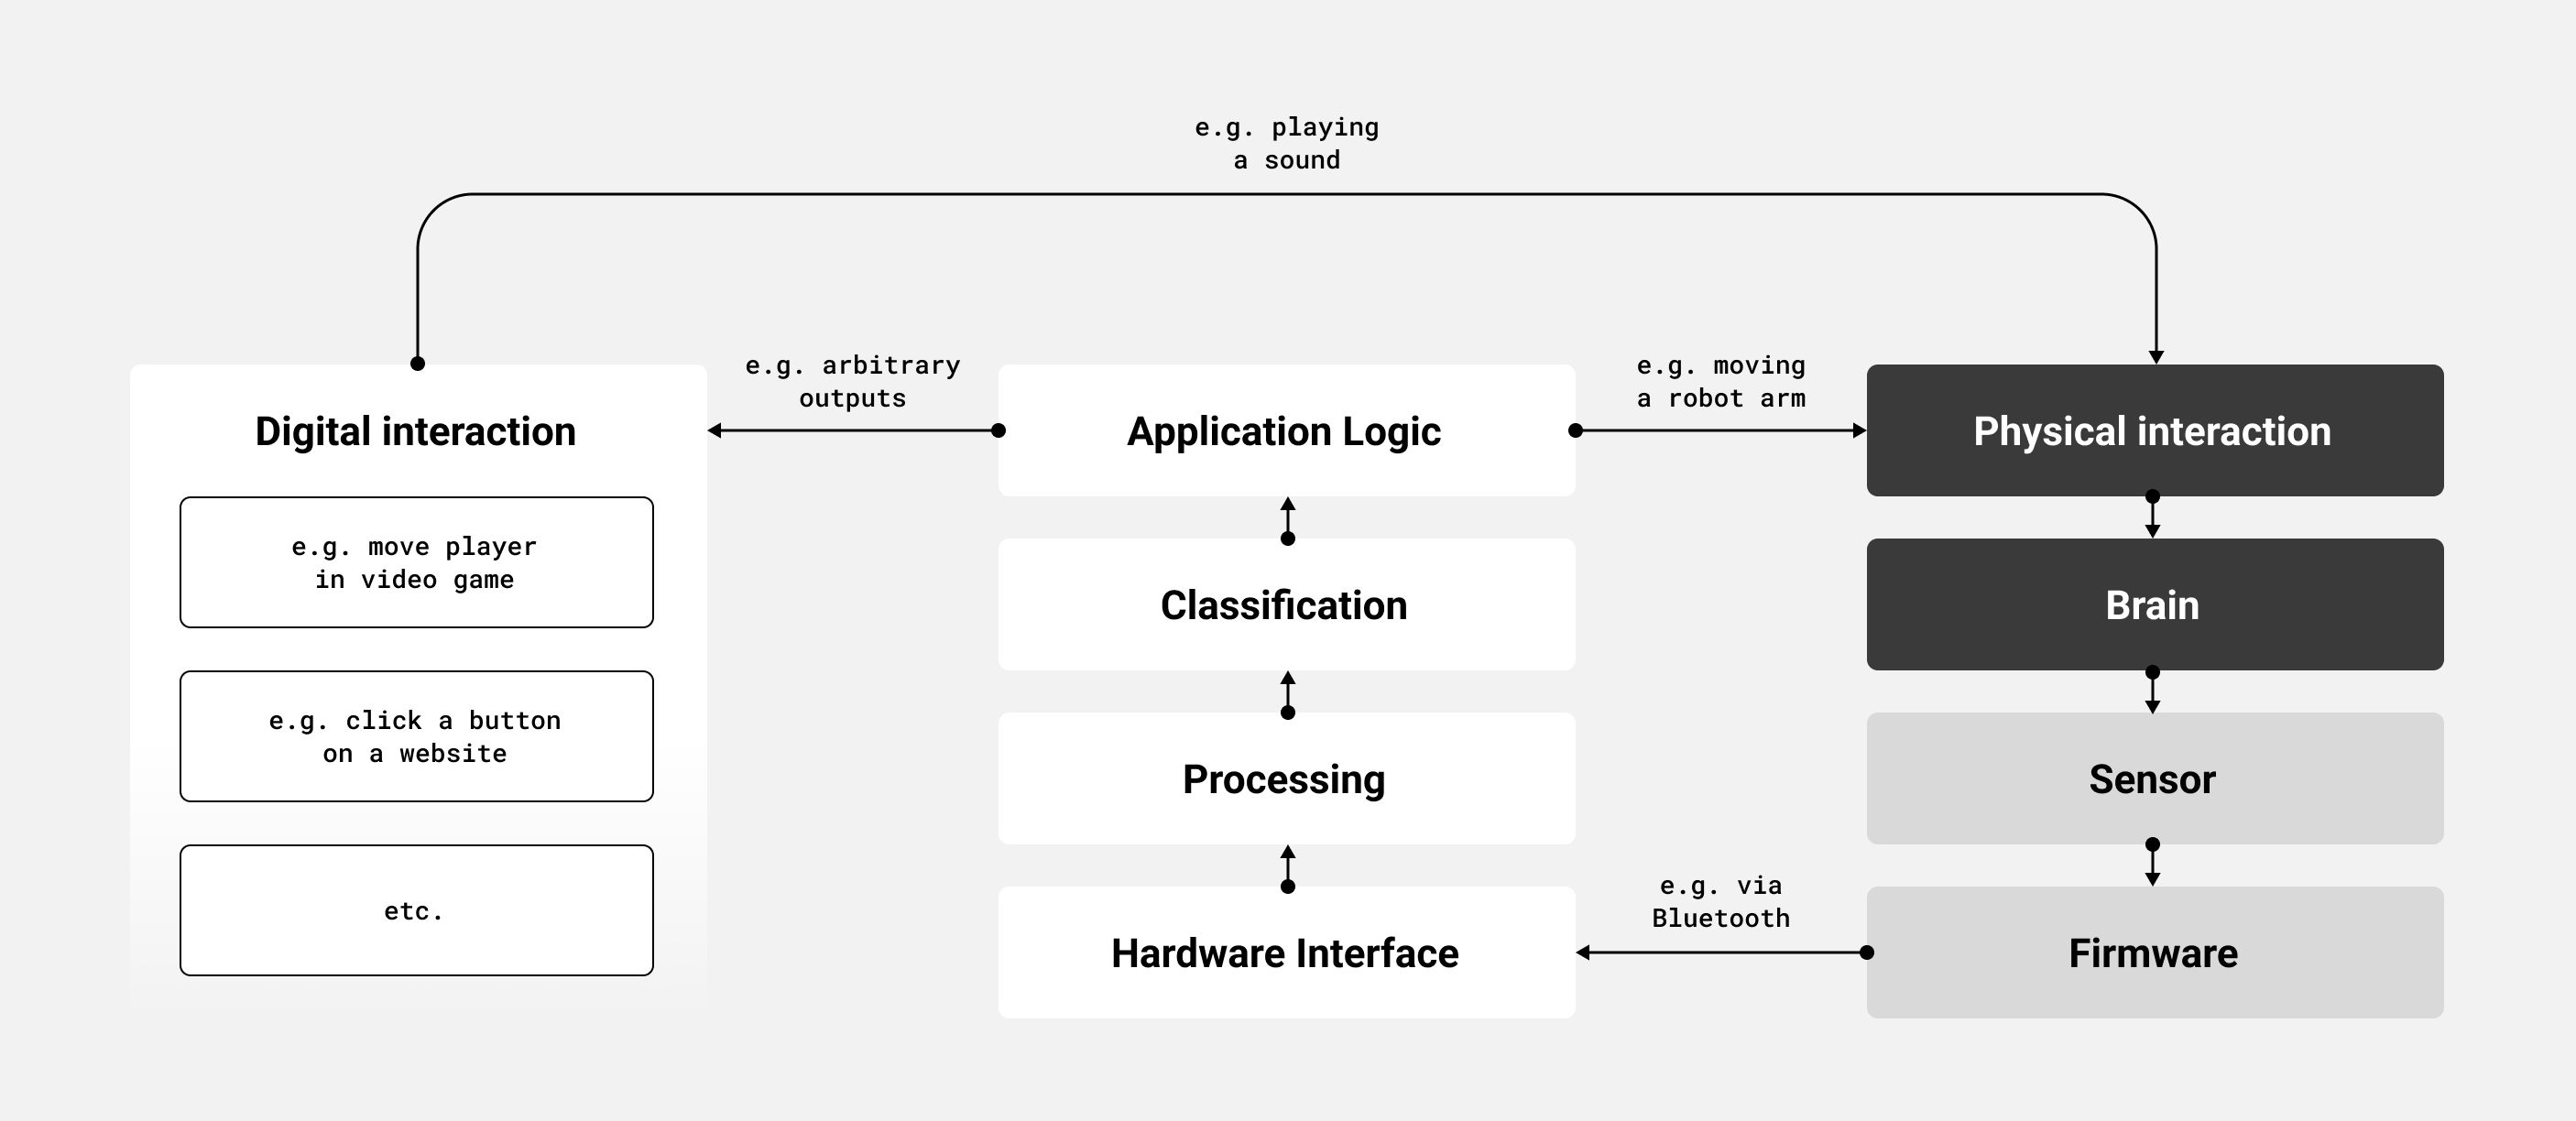
\includegraphics[width=\linewidth]{bci-components.png}
  \caption{Architectural overview of BCI components including a bidirectionality due to neurofeedback in form of e.g. playing a sound in a certain frequency to enable SSVEP (own representation, 2022).}
  \label{fig:bci-components}
\end{figure}

As shown on \autoref{fig:bci-components}, a BCI's two primary components are the hardware and the software. Next to the hardware, there is also the physical part of it, e.g. the brain and a physical interaction counterpart in the form of, e.g. a robot arm\footnote{Some people call this a brain-machine interface rather than a brain-computer interface because you interface with a machine rather than a computer.}. The software is the part that is responsible for the actual processing of the data, e.g. extracting the relevant information from the raw data and turning it into a meaningful output that the application layer can use. The application layer interacts then with a physical or digital counterpart to, e.g. move a player in a game or start playing sound on the computer via its speakers.

\subsection{Unobtrusive hardware and software}
\label{chapter2-unobtrusive-hardware-and-software}

The unobtrusiveness of hardware and software is another aspect to consider when discussing BCIs. Unobtrusiveness in hardware means that it is either not visible at all\footnote{There are other things related to the overall user experience (UX) that are sometimes included in the notion of unobtrusiveness, such as comfort, reusability and convenience, where the author only implies physical characteristics such as shape and size}, such when sensors are implanted beneath the skull, or that it is in a form factor that is already socially accepted, such as glasses or headphones. The prototype of IDUN Technologies' hardware, which measures brain activity in the ear canal, is shown in \autoref{fig:unobstrusive-hardware} that aims to resemble in-earbuds. \autoref{fig:obstrusive-hardware} shows the Neurosity device, which measures brain activity on the head and is not comparable to a socially established form factor. What is considered socially established and accepted truly depends on the society and context, as one could argue that wearing a Neurosity device under a hat while talking to a friend is more acceptable than wearing in-earbuds. However, if, for example, in-ear EEG technology is becoming more discreet, such as hearing aids, it is more inconspicuous and socially acceptable.

\begin{figure}[!htb]
  \minipage{0.49\textwidth}
  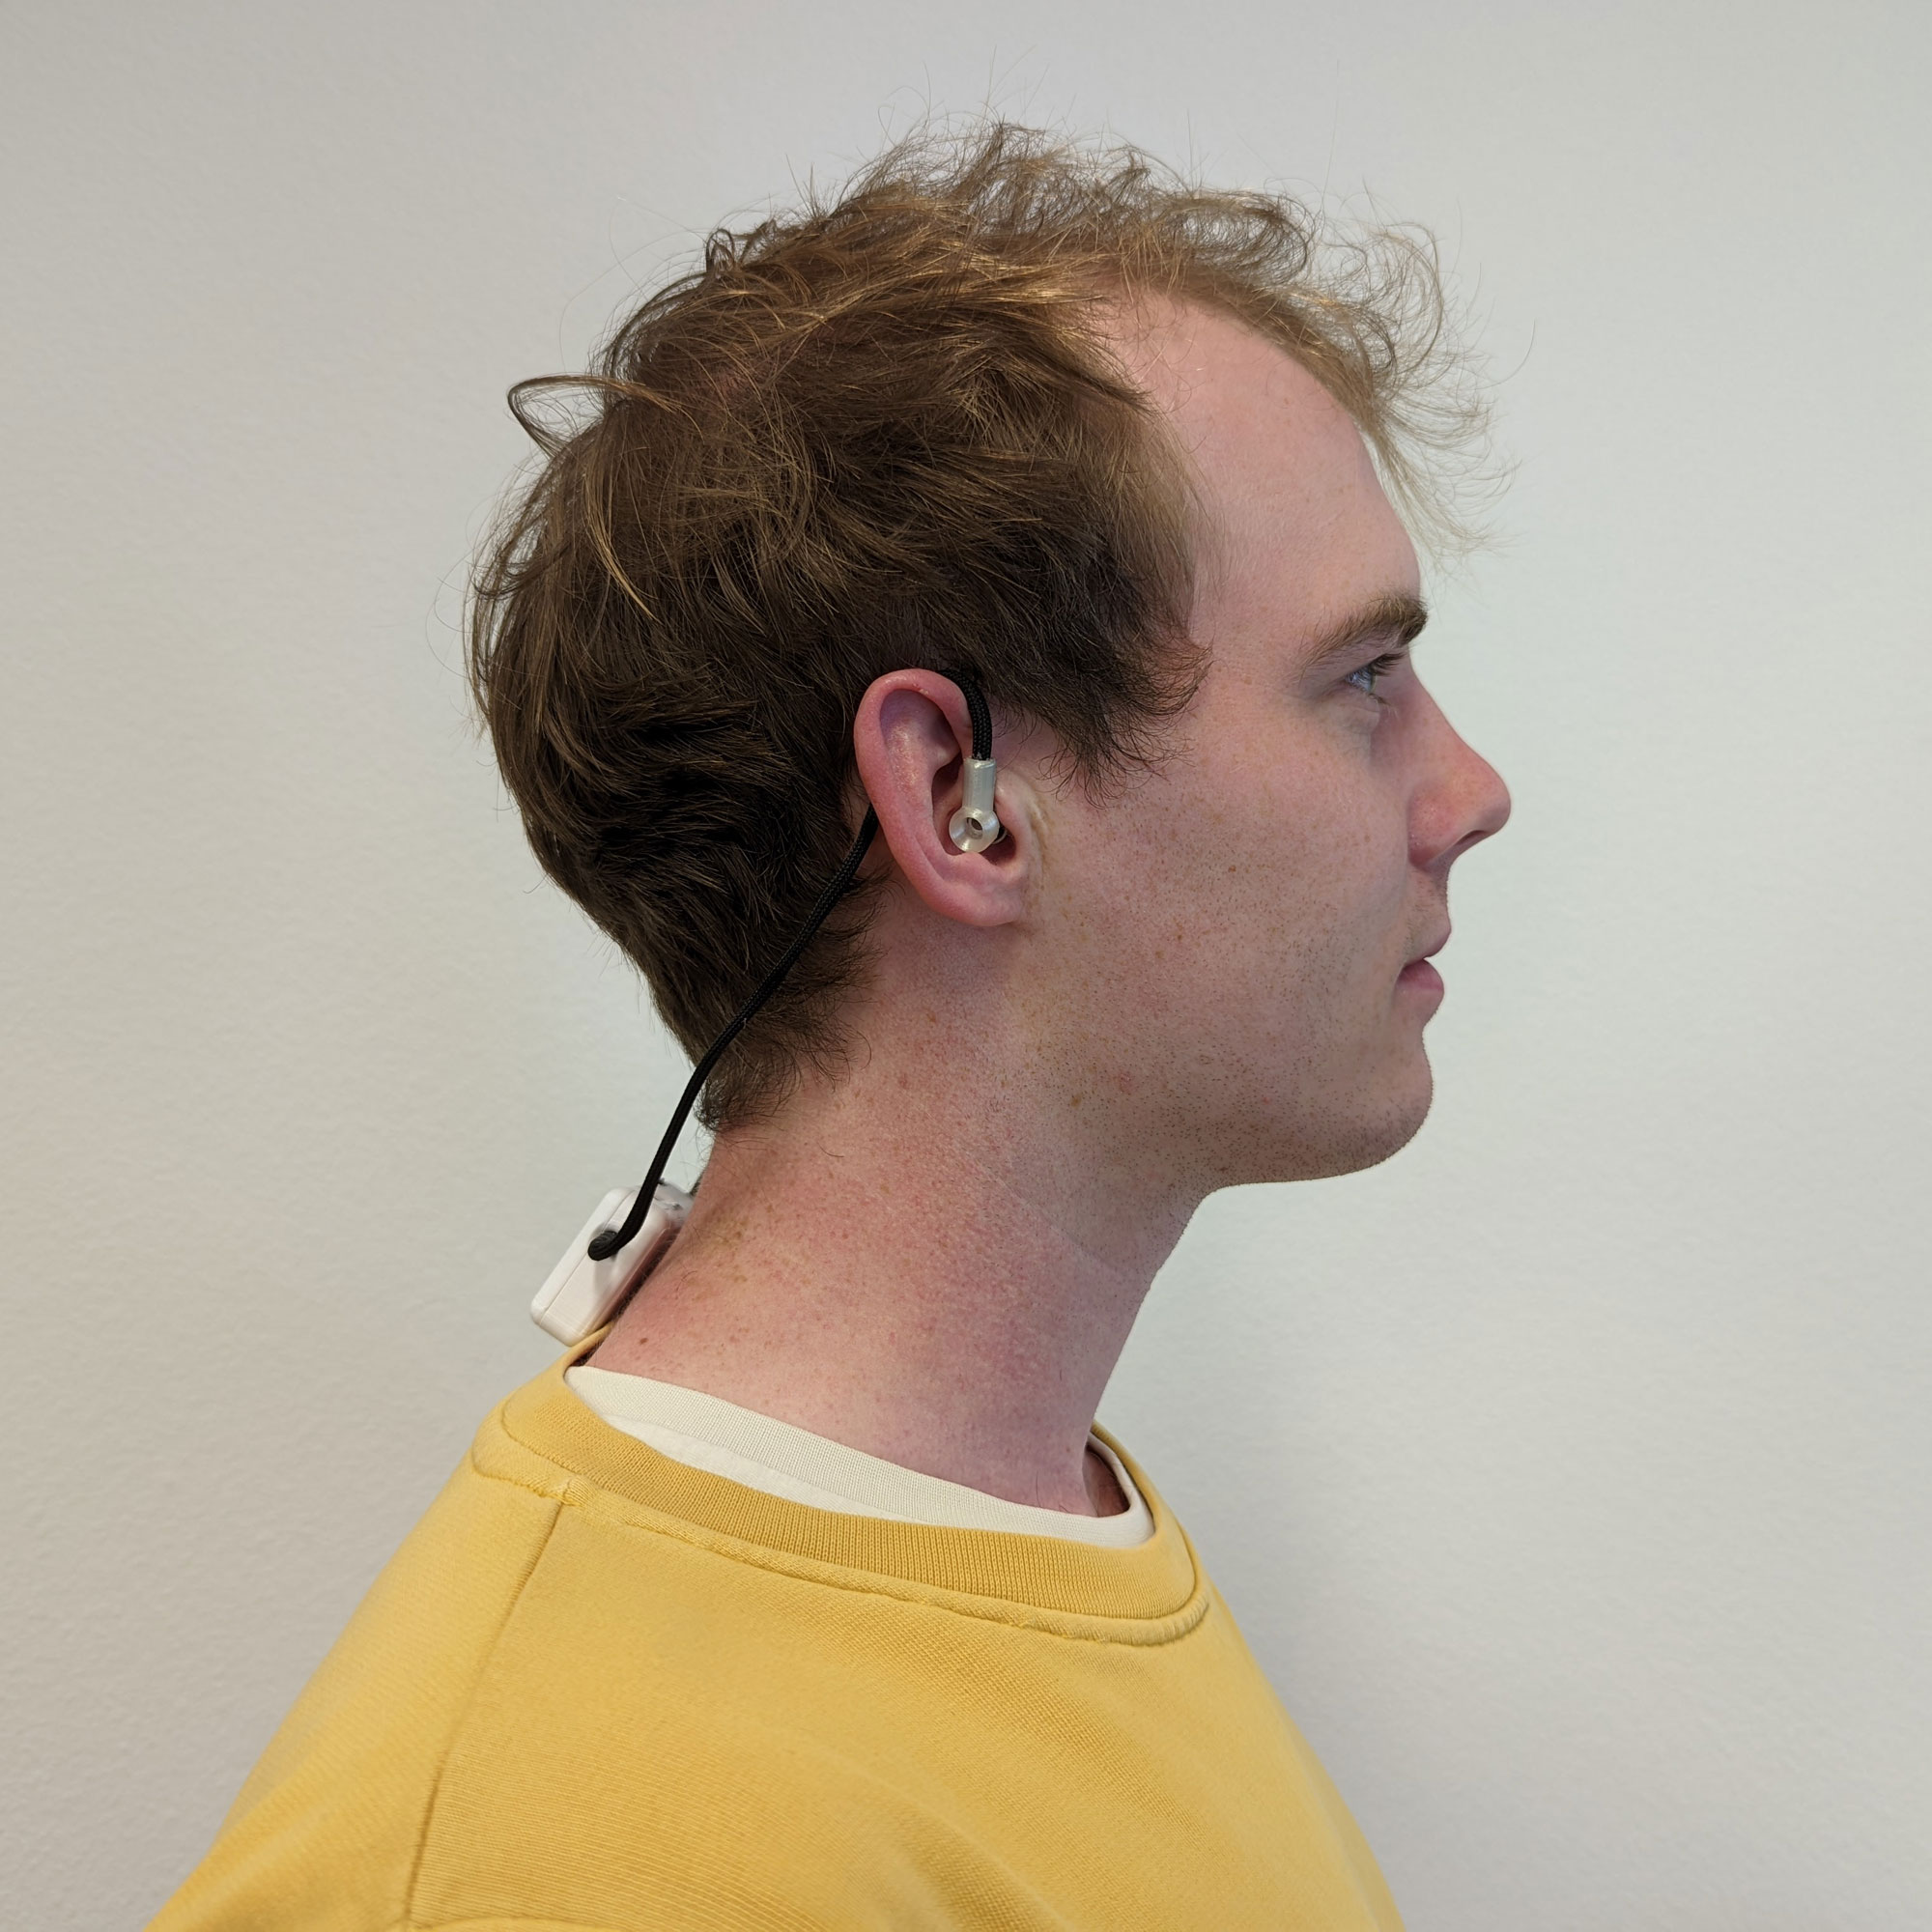
\includegraphics[width=\linewidth]{unobtrusive.jpg}
  \caption{IDUN Guardian hardware, \\ unobtrusive BCI (own representation, 2022).}
  \label{fig:unobstrusive-hardware}
  \endminipage\hfill
  \minipage{0.49\textwidth}
  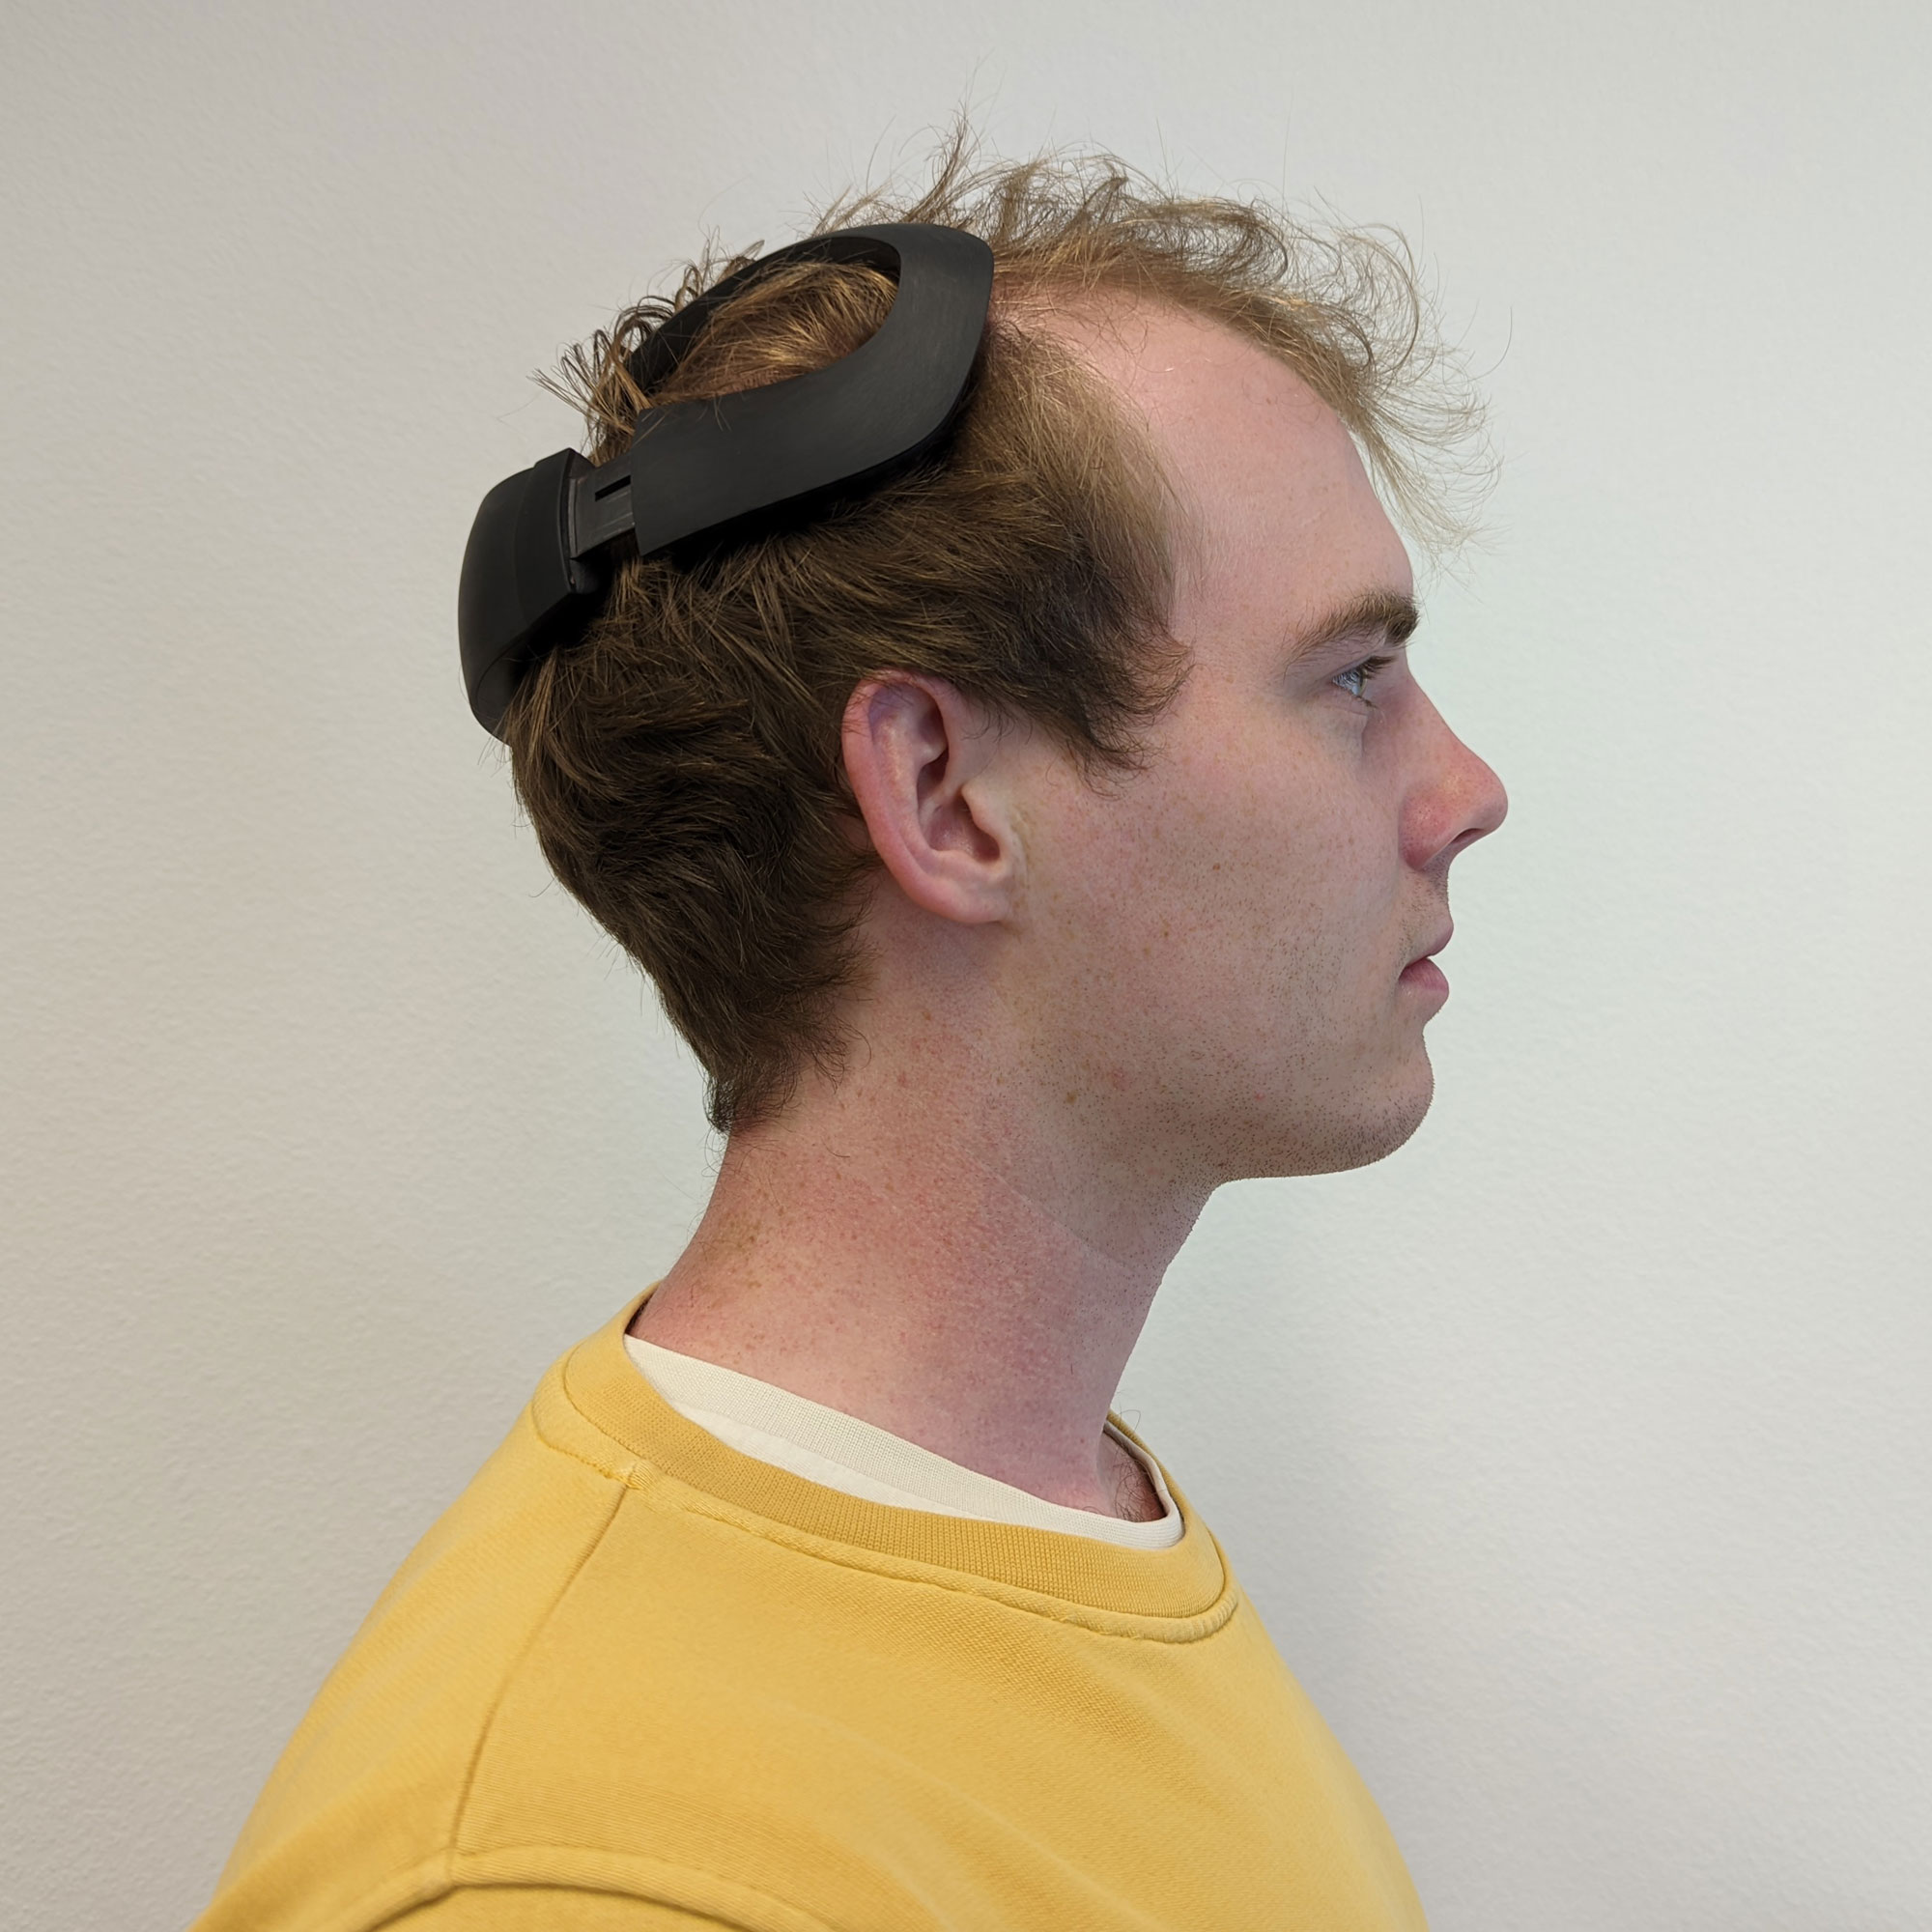
\includegraphics[width=\linewidth]{obtrusive.jpg}
  \caption{Neurosity Notion hardware, \\ obtrusive BCI (own representation, 2022).}
  \label{fig:obstrusive-hardware}
  \endminipage\hfill
\end{figure}

The implications of different form factors must also be considered, such as the possibility of moving the device and thus creating motion artefacts in the signals or the position of the sensors. The ear canal, for example, is ideally closely located to the brain's auditory cortex but not so much for the visual cortex, which is located at the back of the head. However, further hardware implications for BCIs are not a topic covered in this thesis.

It is perhaps not as simple to discuss the unobtrusiveness of software as it is with hardware. Unobtrusive\footnote{Other words for unobtrusive could be discreet, fully-integrated, invisible or simply "in the background".} software, as defined by the author, is the abstraction of the underlying software or system that executes the logic to fulfil a task without the user knowing what the technical requirements are. As an example: To use an HP ENVY Photo 6200 printer with one's Android phone, one must first download the HP Smart app and the HP Print Service Plugin app that acts as a driver for the printer in order to get it set up and running \citep{hp_hp_nodate}. In the case of the HP printer, the user must understand some of the underlying technical requirements in order for it to work, rather than simply concentrating on the task of printing something. For example, unobtrusive software is when one gets a new computer mouse that they simply plug in and it works\footnote{unobtrusiveness usually correlates with usability, but it is not always the case, e.g. more advanced users would not consider locked-in abstraction as more usable. Therefore, the aspect of usability (as well as accessibility) always remains context-bound.}.

Unobtrusive software in BCI refers to the ability to connect one's hardware to the computer or smartphone and use it without the need for additional software such as drivers or command-line interface (CLI) software. As an example: To use an OpenBCI device, one needs to open the GUI app, connect the hardware, test its quality, begin a data stream session, output the stream as, e.g. a Lab Streaming Layer (LSL) or via the User Datagram Protocol (UDP), connect to the signal from, e.g. Neuromore Studio \citep{openbci_neuromore_nodate}, run the data through a classification pipeline, and then connect the output from Neuromore to a video game via the engine itself to have controls for the video game. It should go without saying that this is not unobtrusive software.

There are examples of software that is included as an executable file and thus is relatively unobtrusive, but the software is closely linked with the hardware and the brand behind the hardware, or it is in the proof of concept (PoC) stage rather than a production-ready application. Buying a new pair of headphones and plugging them into one's computer to enjoy neuro-enhanced\footnote{Neuro-enhanced in the context of applications and software can be described as adding additional features to input methods via the brain, e.g. brain commands rather than typing or mouse clicking.} experiences that interact with the brain's outputs or measure brain data across all apps and the operating system would be an example of proper unobtrusive software. One step in this direction would mean to create standards such as a shared understanding of a N/CI or, in general, to come out of the PoC stage of most BCI software and instead create extensible and production-ready software.

\newpage
\subsection{Production-grade software}
\label{chapter2-production-grade-software}

There is no textbook definition of what production-grade software is, but in most cases, software developers agree on the following points:

\begin{itemize}
  \item The software works at any time when access is required. It is therefore capable of frequent and intensive use in commercial or industrial environments.
  \item Software whose behaviour is deterministic and predictable and is, therefore, well-tested, well-documented and optimised in terms of speed, efficiency and security for the given context (e.g. the size of the user base). Usually, developers agree on a Definition of Done (DoD) inside their team to what is considered production-ready, e.g., test coverage of 80+\%, peer-reviewed and commented code, and a common code style guide, to name a few.
  \item Software that runs in a production environment, i.e. on a cloud computing cluster for actual users rather than in a test environment with test users or, for example, on hardware delivered to real customers, and that can adapt itself to the context, e.g. to a higher access rate or insecure user-generated input. In most cases, especially in cloud computing, production-ready also means larger data sets, such as in databases, the possibility of a more significant number of edge cases due to a larger user base, and, most importantly, more available computing power on production instances.
\end{itemize}

As stated in previous sections, most BCIs, such as the OpenBCI, are not intended for production. They are intended for PoCs used in examples, such as controlling objects in games or conducting research. End-to-end and full-stack BCIs for production are rare, as most are very specific and not intended for general purposes, such as the Muse headband, or the software aspect is intended for PoCs or researchers, such as with Emotiv. Pure software products, such as Neuromore, lack the hardware component and miss, for example, an SDK that can be integrated into existing software for different platforms. Neurosity, for example, the company behind the device depicted in \autoref{fig:obstrusive-hardware}, aims to provide a universally usable and unobtrusive software stack that is even open-source. However, because the hardware is not unobtrusive enough, it does not qualify the author's definition as production-ready (apart from the fact that it is not known whether their software stack is aimed to be used in production \citep{neurosity_neurosity_2022} or that third-party developers provide disclaimers of being a work in progress \citep{turney_notion_2022}).

\newpage

Companies such as e.g. Neuralink are presumably working on a general-purpose, unobtrusive and production-ready software system which enables developers to build production apps and even platforms on top of it for a variety of use cases without being limited \citep{musk_integrated_2019}, in their case, since it is a bidirectional BCI, developers are also able to write data back to the brain. Since their aimed hardware is also as unobtrusive in the form factor (since it is implanted), they have a high potential to become one of the first mass-market-ready BCIs if we ignore the fact that we need surgery to get the device itself \citep{neuralink_approach_nodate} and other considerations as a harder opt-out of the device compared to, e.g. plugging out earphones.

\section{Neural/cloud interface definition}
\label{chapter2-neural-cloud-interface-definition}

This section discusses the definition, need and differentiation of a N/CI and the paradigm shifts associated with it when discussing BCI software.

\subsection{BCI software on the cloud}
\label{chapter2-bci-software-on-the-cloud}

Looking at \autoref{fig:nci-components}, we can see that the three software layers of a BCI-component illustration, as pictured on \autoref{fig:bci-components} are highlighted. This is because these components can run on the cloud, i.e. on a public cloud provider such as Amazon Web Services (AWS).

\begin{figure}[!ht]
  \centering
  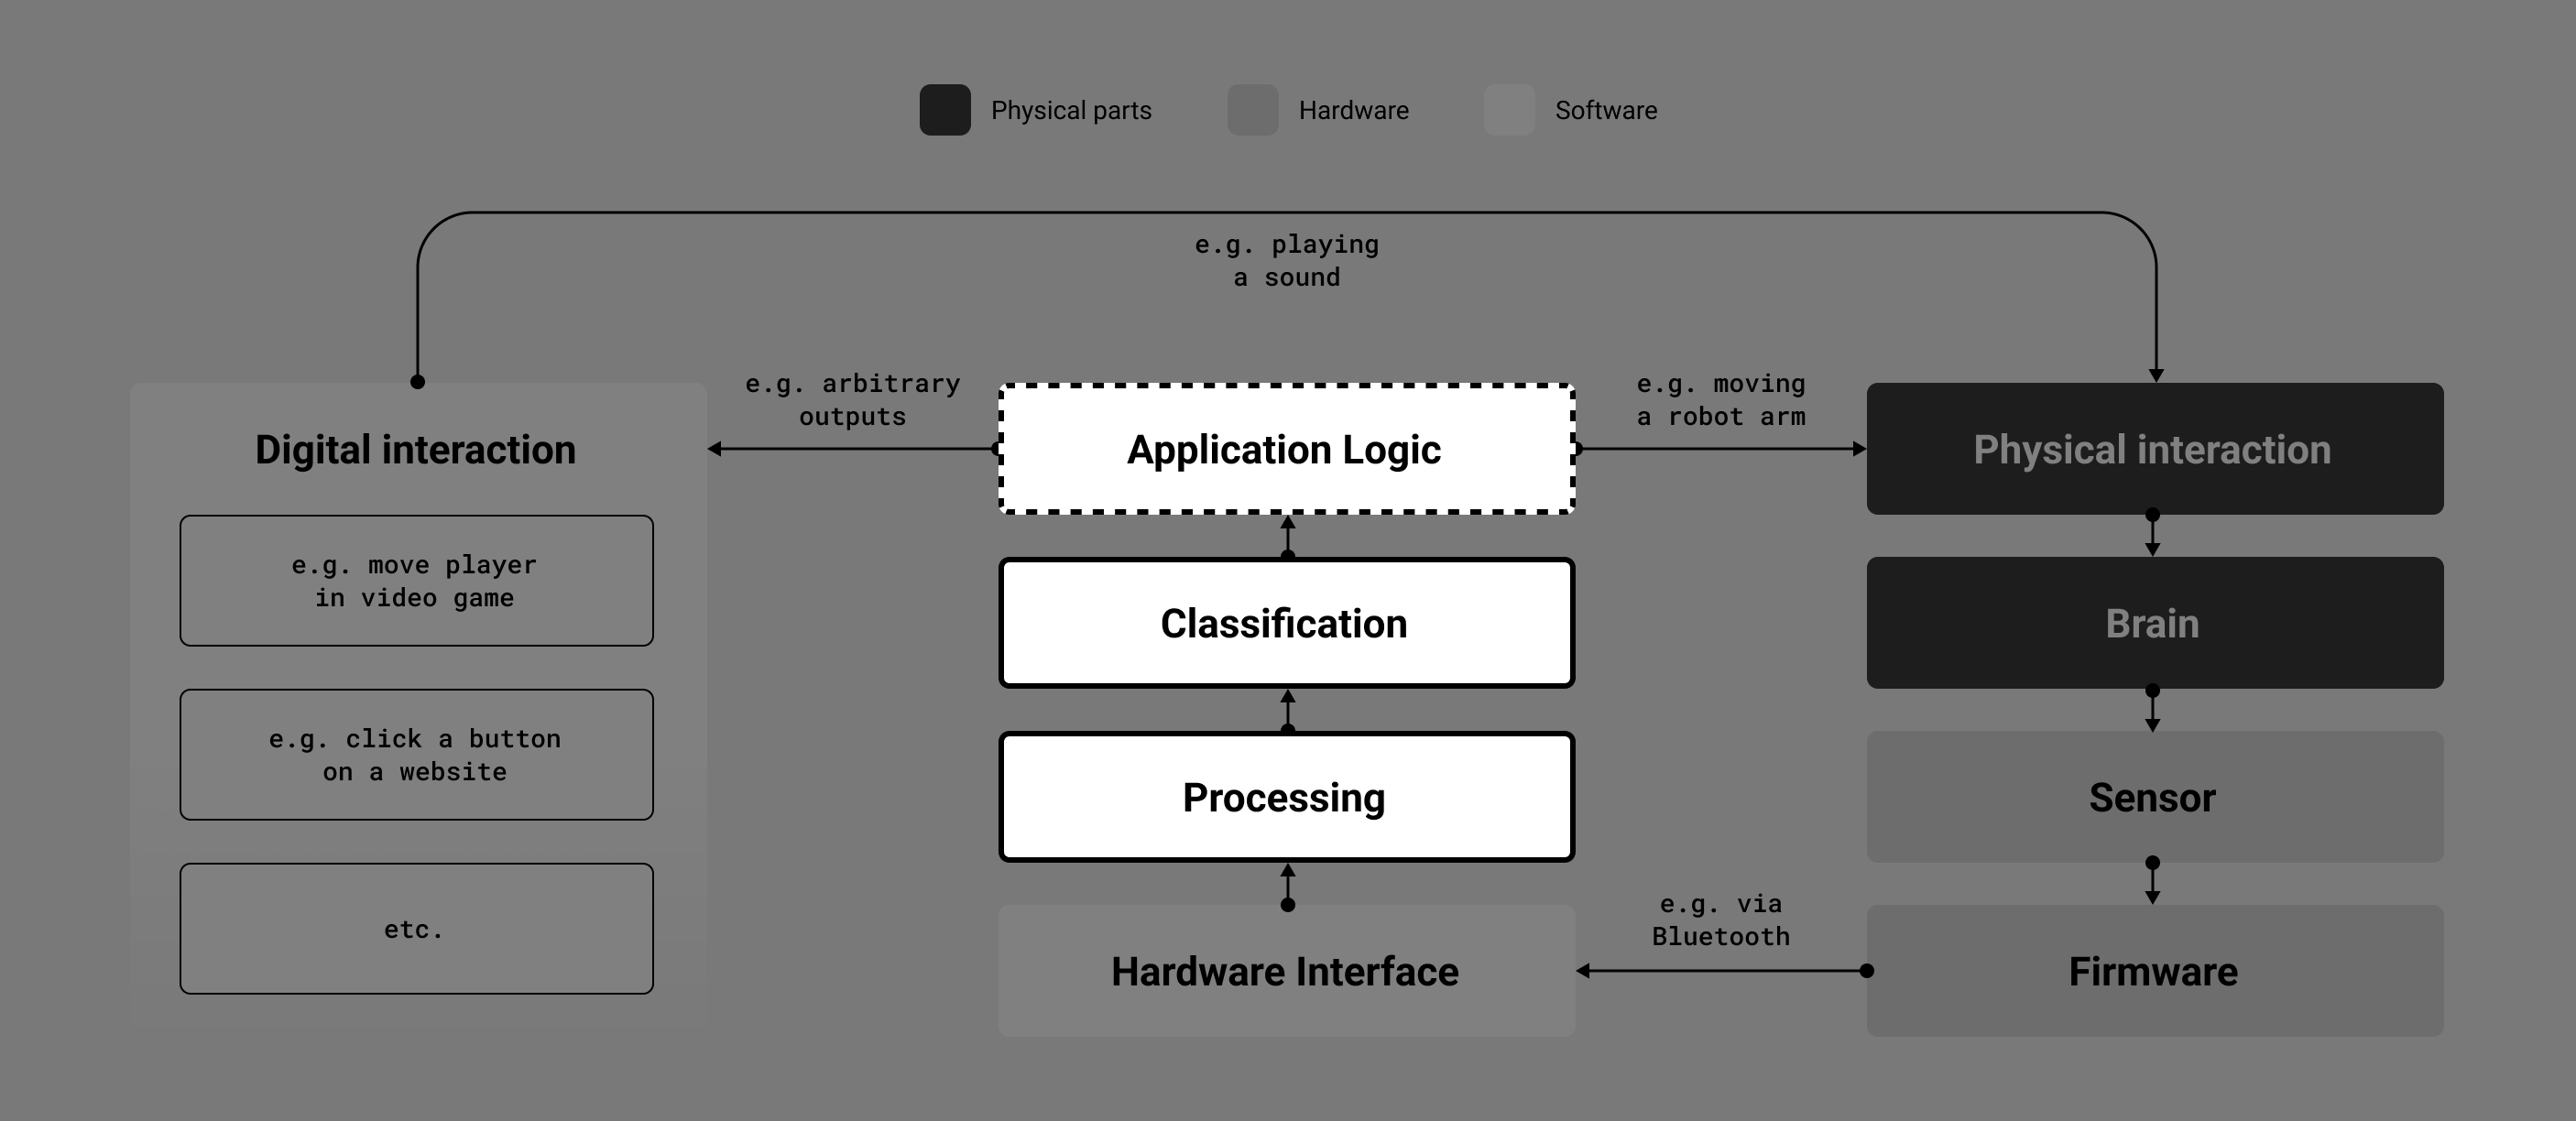
\includegraphics[width=\linewidth]{nci-components.png}
  \caption{Highlight of the software components as shown on \autoref{fig:bci-components} of a BCI that could be moved to the cloud. The Application Logic layer can partially be part of the cloud, but doesn't need to be entirely part if it (own representation, 2022).}
  \label{fig:nci-components}
\end{figure}

Running software on the cloud means that developers or companies can access provisioned information technology (IT) infrastructure through the internet, usually with a pay-as-you-go pricing model \citep{amazon_web_services_inc_what_nodate}. The development speed of software applications can drastically improve since software developers can only focus on software rather than incorporating the hardware and network aspect of setting up their server farms, therefore abstracting the hardware part away. What started with simple computers that can be rented on a server such as it was with, e.g. AWS Elastic Compute Cloud (EC2) \citep{barr_amazon_2006} ended up being a diverse offering from cloud providers with various abstraction levels as shown on \autoref{tab:cloud-computing-types}.

\begin{table}[!ht]
  \centering
  \resizebox{\textwidth}{!}{%
    \begin{tabular}{ll}
      \rowcolor[HTML]{000000}
      {\color[HTML]{FFFFFF} Type}                                                                                 &
      {\color[HTML]{FFFFFF} Description}                                                                                                                                                                                                                                                                                                                           \\ \hline
      \multicolumn{1}{|l|}{\textbf{\begin{tabular}[c]{@{}l@{}}Infrastructure as\\ a Service (laaS)\end{tabular}}} &
      \multicolumn{1}{l|}{\begin{tabular}[c]{@{}l@{}}IaaS gives access to data storage space, virtual or dedicated\\ computers, and network services. The greatest degree of\\ flexibility and administrative control over your IT resources\\ are provided by utilising IaaS.\end{tabular}}                                                                       \\ \hline
      \multicolumn{1}{|l|}{\textbf{\begin{tabular}[c]{@{}l@{}}Platform as a\\ Service (PaaS)\end{tabular}}}       &
      \multicolumn{1}{l|}{\begin{tabular}[c]{@{}l@{}}PaaS lets developers concentrate on developing and\\ managing their code rather than worrying about the\\ underlying infrastructure (often hardware and operating\\ systems). An example is Kubernetes.\end{tabular}}                                                                                         \\ \hline
      \multicolumn{1}{|l|}{\textbf{\begin{tabular}[c]{@{}l@{}}Software as a\\ Service (SaaS)\end{tabular}}}       &
      \multicolumn{1}{l|}{\begin{tabular}[c]{@{}l@{}}SaaS provides a whole product that is run and controlled \\ by the service provider. The phrase SaaS often refers to\\ end-user apps (e.g. web-based email). Developers don't\\ have to be concerned about how the service is handled\\ or whether the underlying infrastructure is maintained.\end{tabular}} \\ \hline
    \end{tabular}%
  }
  \vspace{10pt}
  \caption{The three abstraction levels and types of cloud computing \citep{amazon_web_services_inc_what_nodate}.}
  \label{tab:cloud-computing-types}
\end{table}
\raggedbottom

The majority of businesses are anticipated to embrace a cloud-first strategy by 2025, according to Milind Govekar, vice president of IT research and consultancy company Gartner, and will not be able to fully implement their digital plans without the usage of cloud-native architectures and technologies \citep{gartner_gartner_nodate}. The impact and importance of cloud computing cannot be underestimated, and its success is also reflected in the annual spending on cloud computing resources, estimated at €474 billion in 2022 \citep{gartner_gartner_nodate}. Cloud computing is such an extensive and complex topic that it could quickly fill entire books. In the following list, the author categorises three essential points from a bird's eye view that certainly plays a vital role in BCI software: 1. Dedicated and deterministic environments, which explains that an environment of a software programme always stays the same independent of the end-users hardware, 2. elastic and high-performance availability, which explains cloud computers that have an on-demand and adjustable high-performance and 3. provided services for speed, which explains the concept of pre-made and dedicated software written primarily for the cloud and specific use cases.

\begin{itemize}
  \item \textbf{Dedicated and deterministic environments:} Running code for BCIs on different end-user platforms, such as Windows or Android, can have drawbacks because each device has its processor, graphics card, operating system version and drivers, which can make developing software that requires stable and good performance, such as a neural data processing pipelines, time-consuming and difficult to maintain, as developers must keep track of every factor of the end-user devices. This is fine for BCIs that are not intended for the general public, such as specially designed BCIs for people with, say, locked-in syndrome, but for the general public, a variety of different end-user devices come into play. When code is run on a dedicated machine, such as a cloud computer with clearly defined hardware and operating system specifications, it becomes less error-prone and more deterministic. The use of virtual machines (VMs) or containerisation on end-user devices attempts to solve this problem but has additional drawbacks beyond this thesis's scope. Most notable is the drawback of being bound to the end-users device performance, which varies from user to user.
  \item \textbf{Elastic and high-performance availability:} Because the cloud model usually runs as an as-needed model, the initial purchase cost of computer hardware is split and shared across usage. Developers have access to tremendous computing power that would not be easily afforded if purchased independently. As a result, when developing a computationally intensive algorithm, developers can use high-performance central processing units (CPUs) and graphics processing units (GPUs) to complete tasks much faster than consumer hardware on end-user devices. Performance can also be increased as needed, for example, to handle heavier tasks that are not used as frequently or to handle more requests when, for example, the demand for the software increases due to an increase in the number of users, which is a process known as elasticity \citep{gartner_definition_nodate}. Furthermore, the cloud provides far more storage capacity than end-user devices. End-users would request more data as needed, which would then be downloaded to their device via the internet, rather than all of the data filling up their storage capacity.

  \item \textbf{Provided services for speed:} The vast majority of cloud providers are providing more specialised services as we move closer to PaaS. Provisioned database servers, for example, exist solely to serve as a database, so the underlying hardware is optimised for the database software running on it, such as, e.g. PostgreSQL. Hundreds of cloud computing services are available, including 200 from AWS alone \citep{amazon_web_services_inc_what_nodate}, all of which address specific use cases. This is extremely useful when it comes to cloud-based BCI software. One example is the aspect of live streaming of brain data, which we will go over in greater detail in the implementation chapter of this thesis. The services provided accelerate development by eliminating the need for teams to reinvent the wheel repeatedly, and they also provide out-of-the scalability, such as in the serverless model \citep{redhat_what_2022}.
\end{itemize}

A N/CI utilises cloud computing by running certain software components of a BCI system in the cloud as, e.g. shown on \autoref{fig:nci-components}. Multiple BCIs can communicate with each other or with other software or hardware over the internet, enabling remote HCI. \autoref{fig:nci-components} depicts how two or more BCIs can interface with one another using cloud software. The red arrows represent the typical BCI possibility of local HCI. The blue arrow depicts how the person on the left can execute business logic via the cloud over the internet, enabling digital and physical interactions with, e.g. high performance. The green arrow depicts how the person on the right can communicate with their BCI via a N/CI with the person on the left even if they are not in the same geographical location.

\begin{figure}[!ht]
  \centering
  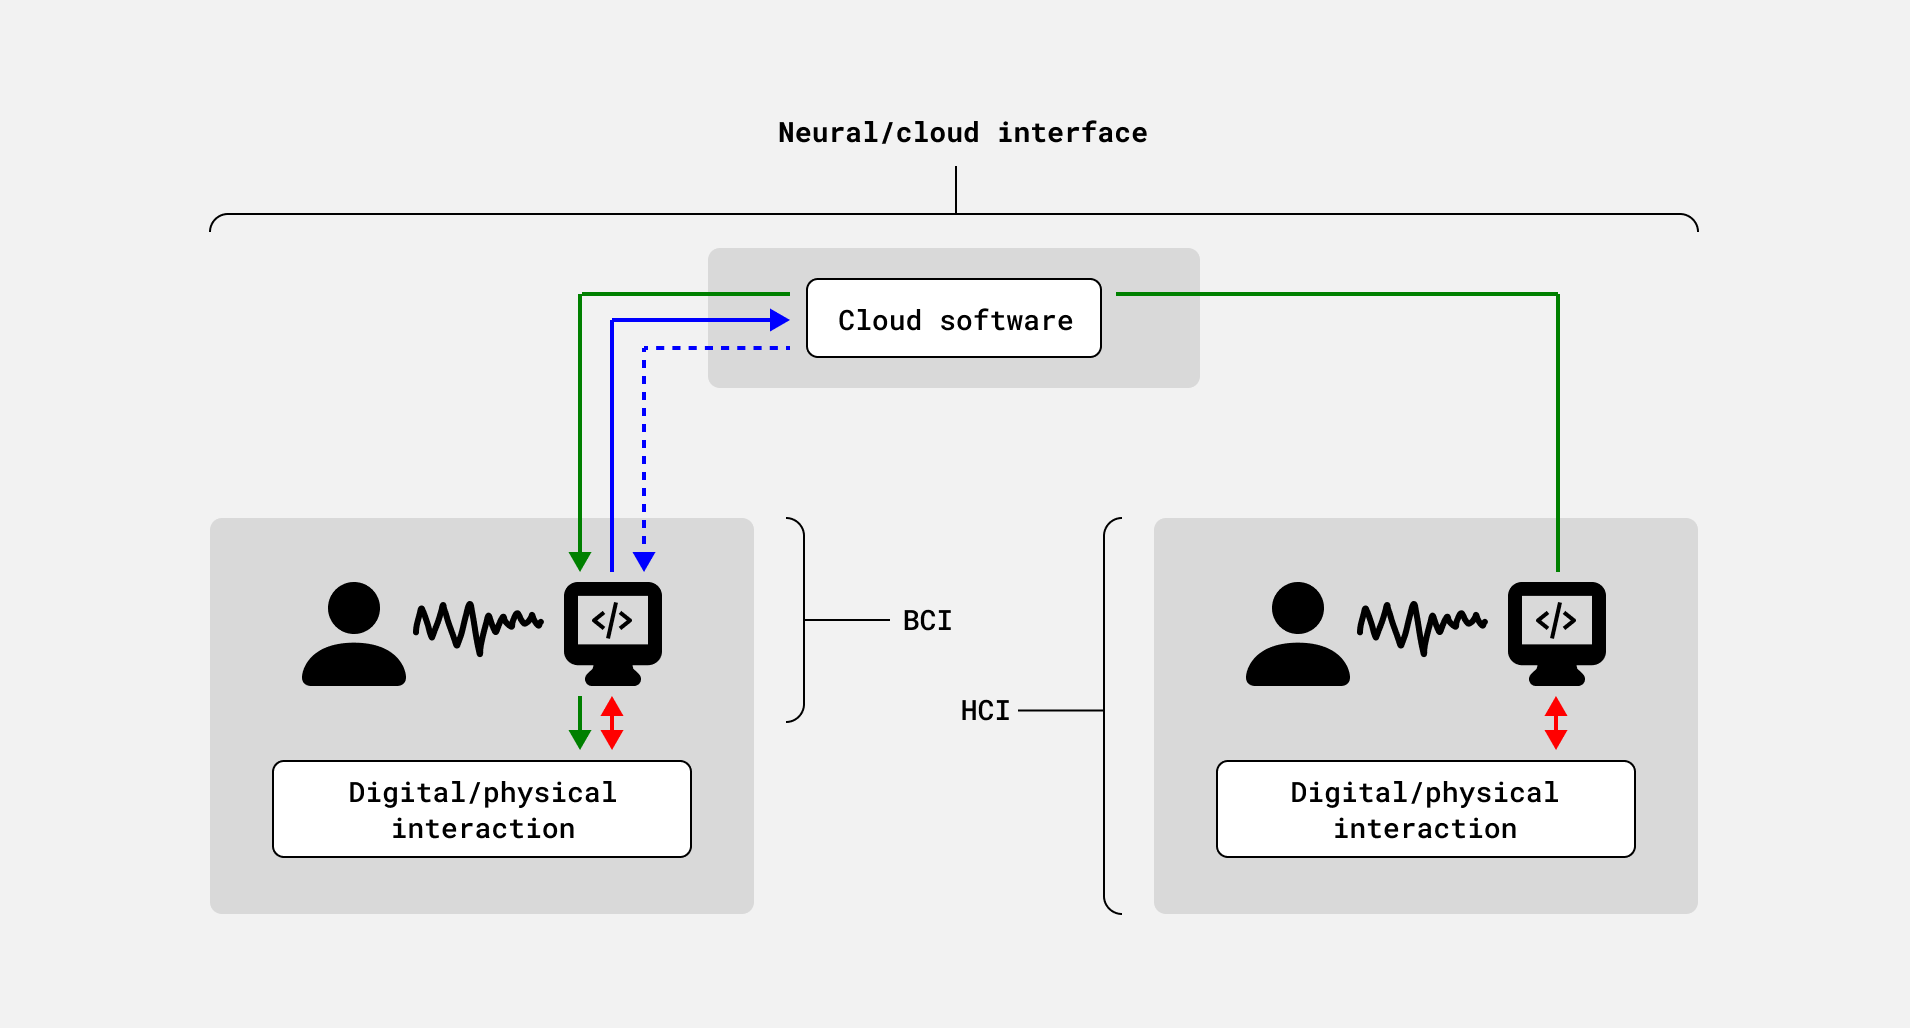
\includegraphics[width=\linewidth]{nci-overview.png}
  \caption{A N/CI is the connection between multiple BCIs (own representation, 2022).}
  \label{fig:nci-overview}
\end{figure}

\subsection{Distinction between existing research}
\label{chapter2-distinction-between-existing-research}

The concept of running BCI software components remotely and on servers is not new and novel, as research into remote BCI, also known as asynchronous or BCI systems, to control Internet of Things (IoT) environments has been ongoing for some time. When we look at the research from \citeauthor{zhang_internet_2018} on their deep learning framework to enable as they describe Human-Thing Cognitive Interactivity, we see a strong emphasis on classification but less on aspects such as scalability and unobtrusiveness, all of which factor in to the more traditional definition of a production-ready system specialised in the communications of multiple BCI software systems \citep{zhang_internet_2018}. \citeauthor{zhang_internet_2018} address latency and the size of EEG samples sent in real-time to a server, as well as the corresponding calculation, but there are no more details in regards to the proposed and very simplified architecture chart's protocols, development operations (DevOps) and effective cloud architecture. Another paper by \citeauthor{ahamad_system_2022} looks at the system architecture of a BCI for IoT, but this time from the perspective of algorithms optimised for time series data such as EEG, with no mention of the effective cloud architecture of such a system \citep{ahamad_system_2022}.

The author introduces the concept of three-dimensionality for the definition of a N/CI based on the previously mentioned topics and research that touch on the issues of this thesis, which are essential to achieve mass adoption for BCIs from the perspective of the software and DevOps engineering for the actual implementation of such a system.

\begin{figure}[!ht]
  \centering
  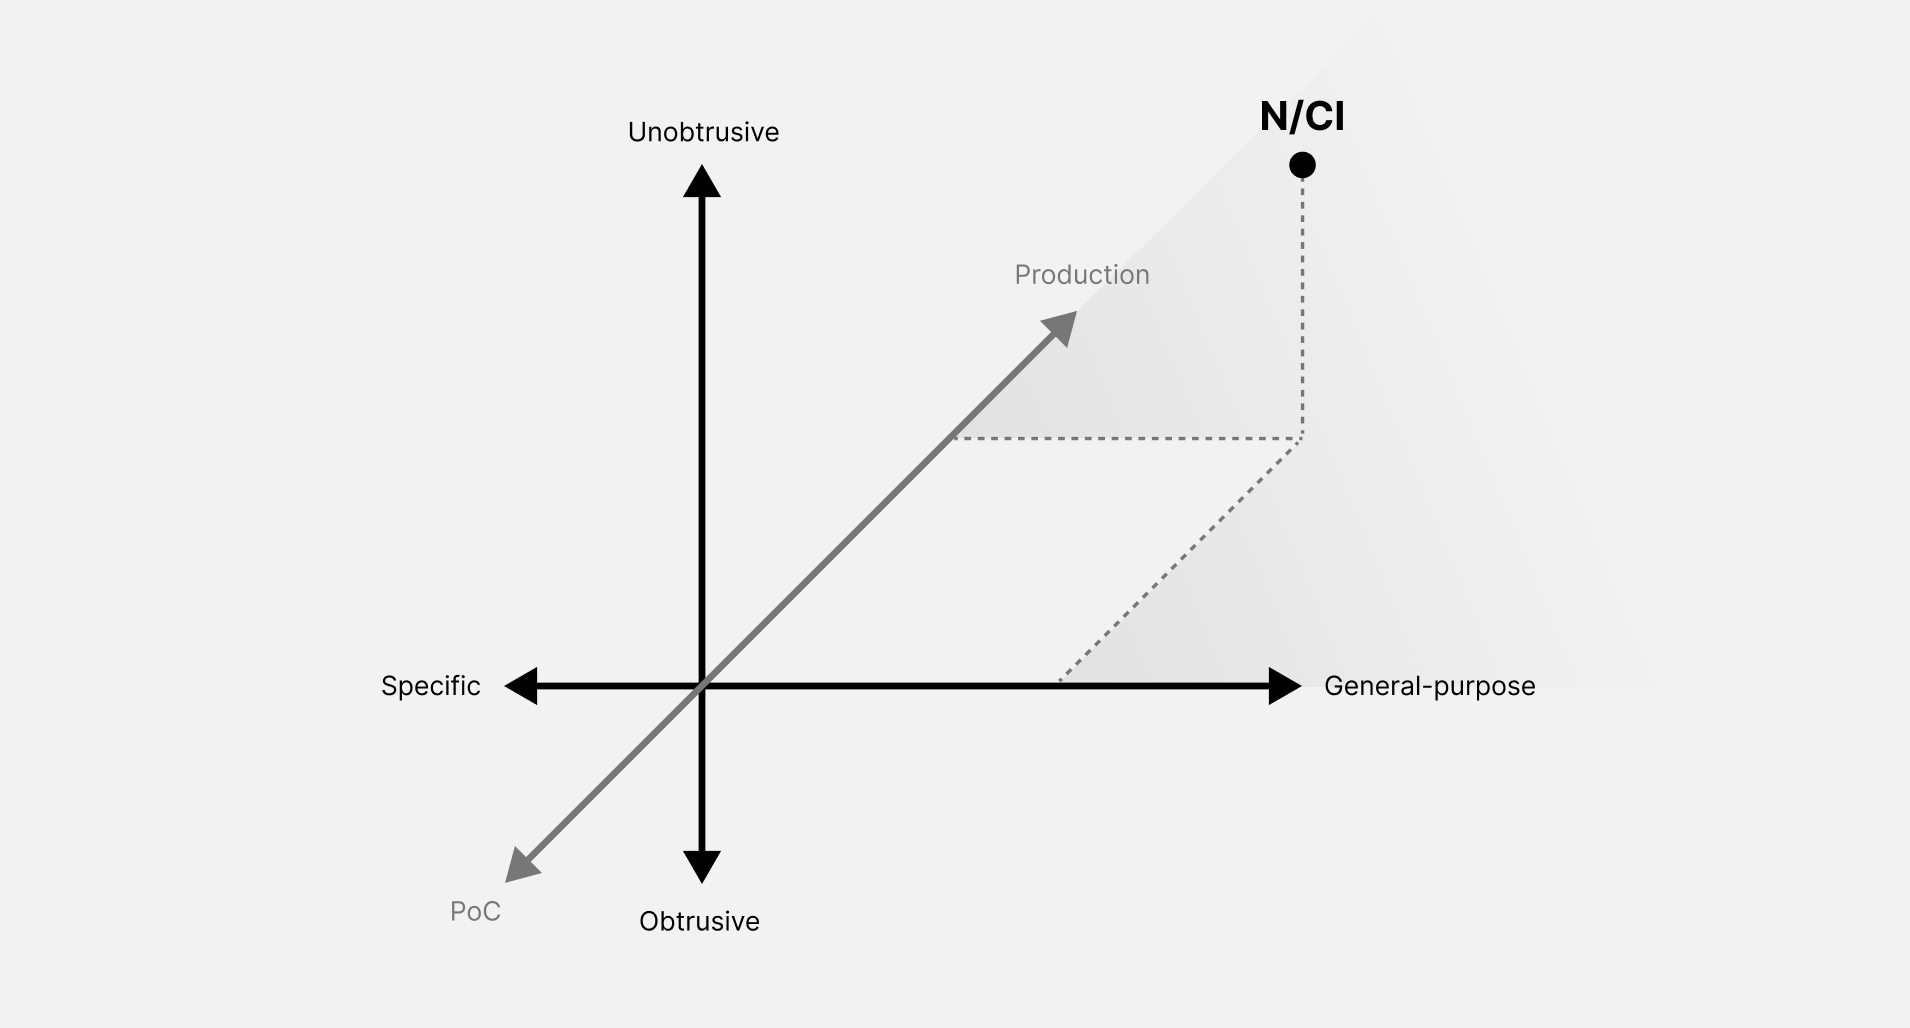
\includegraphics[width=\linewidth]{nci-definition.png}
  \caption{Visualisation of the three-dimensionality of the term neural/cloud interface (own representation, 2022).}
  \label{fig:nci-definition}
\end{figure}

\subsection{Requirements of a N/CI}
\label{chapter2-requirements-of-a-nci}

\autoref{fig:nci-definition} shows three axes and positions the term N/CI in the intersection of a software system that can undoubtedly be defined as production-ready rather than being a proof of concept, unobtrusive implementation rather than obtrusive software and general-purpose applicability rather than being made just for a specific use case. Following on \autoref{tab:nci-axis}, you can see the definitions of the axis descriptions.

% Please add the following required packages to your document preamble:
% \usepackage{graphicx}
% \usepackage[table,xcdraw]{xcolor}
% If you use beamer only pass "xcolor=table" option, i.e. \documentclass[xcolor=table]{beamer}
\begin{table}[!ht]
  \centering
  \resizebox{\textwidth}{!}{%
    \begin{tabular}{ll}
      \rowcolor[HTML]{000000}
      {\color[HTML]{FFFFFF} Axis labelling}                   &
      {\color[HTML]{FFFFFF} Description}                                                                                                                                                                                                                                                                                                                                                                                                                                                                                                                                                                                  \\ \hline
      \multicolumn{1}{|l|}{\textbf{Production}}               &
      \multicolumn{1}{l|}{\begin{tabular}[c]{@{}l@{}}As previously stated, this is the range in which a software system is deemed ready for production.\\ Because the definition is vague, it is difficult to identify specific requirements that must be met for\\ a system to be considered production-ready. However, for a N/CI, this means running in a\\ production environment, e.g. in a cloud, on a real-world end-user server rather than, for example,\\ in a proof-of-concept environment such as in a lab.\end{tabular}}                                                                                     \\ \hline
      \multicolumn{1}{|l|}{\textbf{Unobtrusive}}              &
      \multicolumn{1}{l|}{\begin{tabular}[c]{@{}l@{}}As previously stated, an unobtrusive software system is one in which the end-user does not need\\ to understand the underlying architecture and requirements in order to use the software or even\\ know certain parts of the software system. In the reverse case, users need to install special\\ packages or download additional companion apps. to make a N/CI work on their computer\\ or smartphone is not the aim of the author's definition of a N/CI.\end{tabular}}                                                                                         \\ \hline
      \multicolumn{1}{|l|}{\textbf{General-purpose}}          &
      \multicolumn{1}{l|}{\begin{tabular}[c]{@{}l@{}}A general-purpose software system is one that can be used for a variety of functions. As an\\ example, consider AWS. It is general-purpose, which means that developers can create\\ cloud software on AWS that can be either a financial application or a backend for a mobile\\ application; there are no specific use cases. This means that a N/CI, unlike the NextMind BCI\\ or the Muse headband, should provide general-purpose functionality rather than specific use\\ cases, i.e. it is not limited to a specific set of functions.\end{tabular}}          \\ \hline
      \rowcolor[HTML]{EFEFEF}
      \multicolumn{1}{|l|}{\cellcolor[HTML]{EFEFEF}PoC}       &
      \multicolumn{1}{l|}{\cellcolor[HTML]{EFEFEF}\begin{tabular}[c]{@{}l@{}}A BCI software system that serves as a proof of concept cannot be considered N/CI because\\ it is not intended for production and thus all the effort required to create a production system,\\ such as quality assurance with unit or end-to-end testing, is unnecessary. A PoC system does\\ not usually run in a production environment, as the goal is, for example, to test a specific\\ functionality of a use case rather than to deliver the software to end-users.\end{tabular}}                                                    \\ \hline
      \rowcolor[HTML]{EFEFEF}
      \multicolumn{1}{|l|}{\cellcolor[HTML]{EFEFEF}Obtrusive} &
      \multicolumn{1}{l|}{\cellcolor[HTML]{EFEFEF}\begin{tabular}[c]{@{}l@{}}An obtrusive BCI system, for example, may still be production-ready if it targets specific use cases\\ while remaining unobtrusive because neuroscientists or developers, for example, expect to have\\ access to the underlying software architecture or technical requirements and thus do not want to\\ abstract from it. If it is obtrusive software, such as OpenBCI, this usually means building the\\ production-ready part on top of it is necessary, which does not fit the author's proposed definition\\ of a N/CI.\end{tabular}} \\ \hline
      \rowcolor[HTML]{EFEFEF}
      \multicolumn{1}{|l|}{\cellcolor[HTML]{EFEFEF}Specific}  &
      \multicolumn{1}{l|}{\cellcolor[HTML]{EFEFEF}\begin{tabular}[c]{@{}l@{}}If a BCI system is only used for one use case, such as Muse for sleep and meditation, companies\\ or developers who want to offer a different use case, such as a mind-controlled keyboard with a\\ P300 system will have to reverse engineer Muse's EEG output or use a different BCI hardware\\ that is less specific and closed, and then build their own production-ready and unobtrusive software\\ on top of it.\end{tabular}}                                                                                                         \\ \hline
    \end{tabular}%
  }
  \vspace{10pt}
  \caption{Axes label descriptions of the three-dimensionality for the definition of a N/CI as shown on \autoref{fig:nci-definition}}
  \label{tab:nci-axis}
\end{table}

The assumption that the empirical development of a real N/CI preceded IDUN Technologies is why a N/CI must be located at the intersection of these three areas. The mission of IDUN Technologies is to create a mass-market BCI for everyone. They accomplish this by constructing EEG sensors in the form of in-ear headphones and measuring brain signals from the ear canal \citep{idun_technologies_guardian_nodate}. With an unobtrusive form factor like the one used by IDUN, a significant barrier to mass-market BCI has already been overcome. Furthermore, IDUN intends to provide a business-to-business (B2B) platform, allowing developers and scientists to create software based on IDUN's offering. As a result, IDUN is developing a universal brain programming interface (API) through which developers and scientists can access brain insights. Because IDUN includes this API in end-user applications, it must be production-ready. IDUN focuses on specific use cases at the start of product development, but this is not due to technical constraints but rather a business decision. The device should be generic rather than specific, allowing developers to build any neuro-enhanced application on top of the API.

\begin{figure}[!ht]
  \centering
  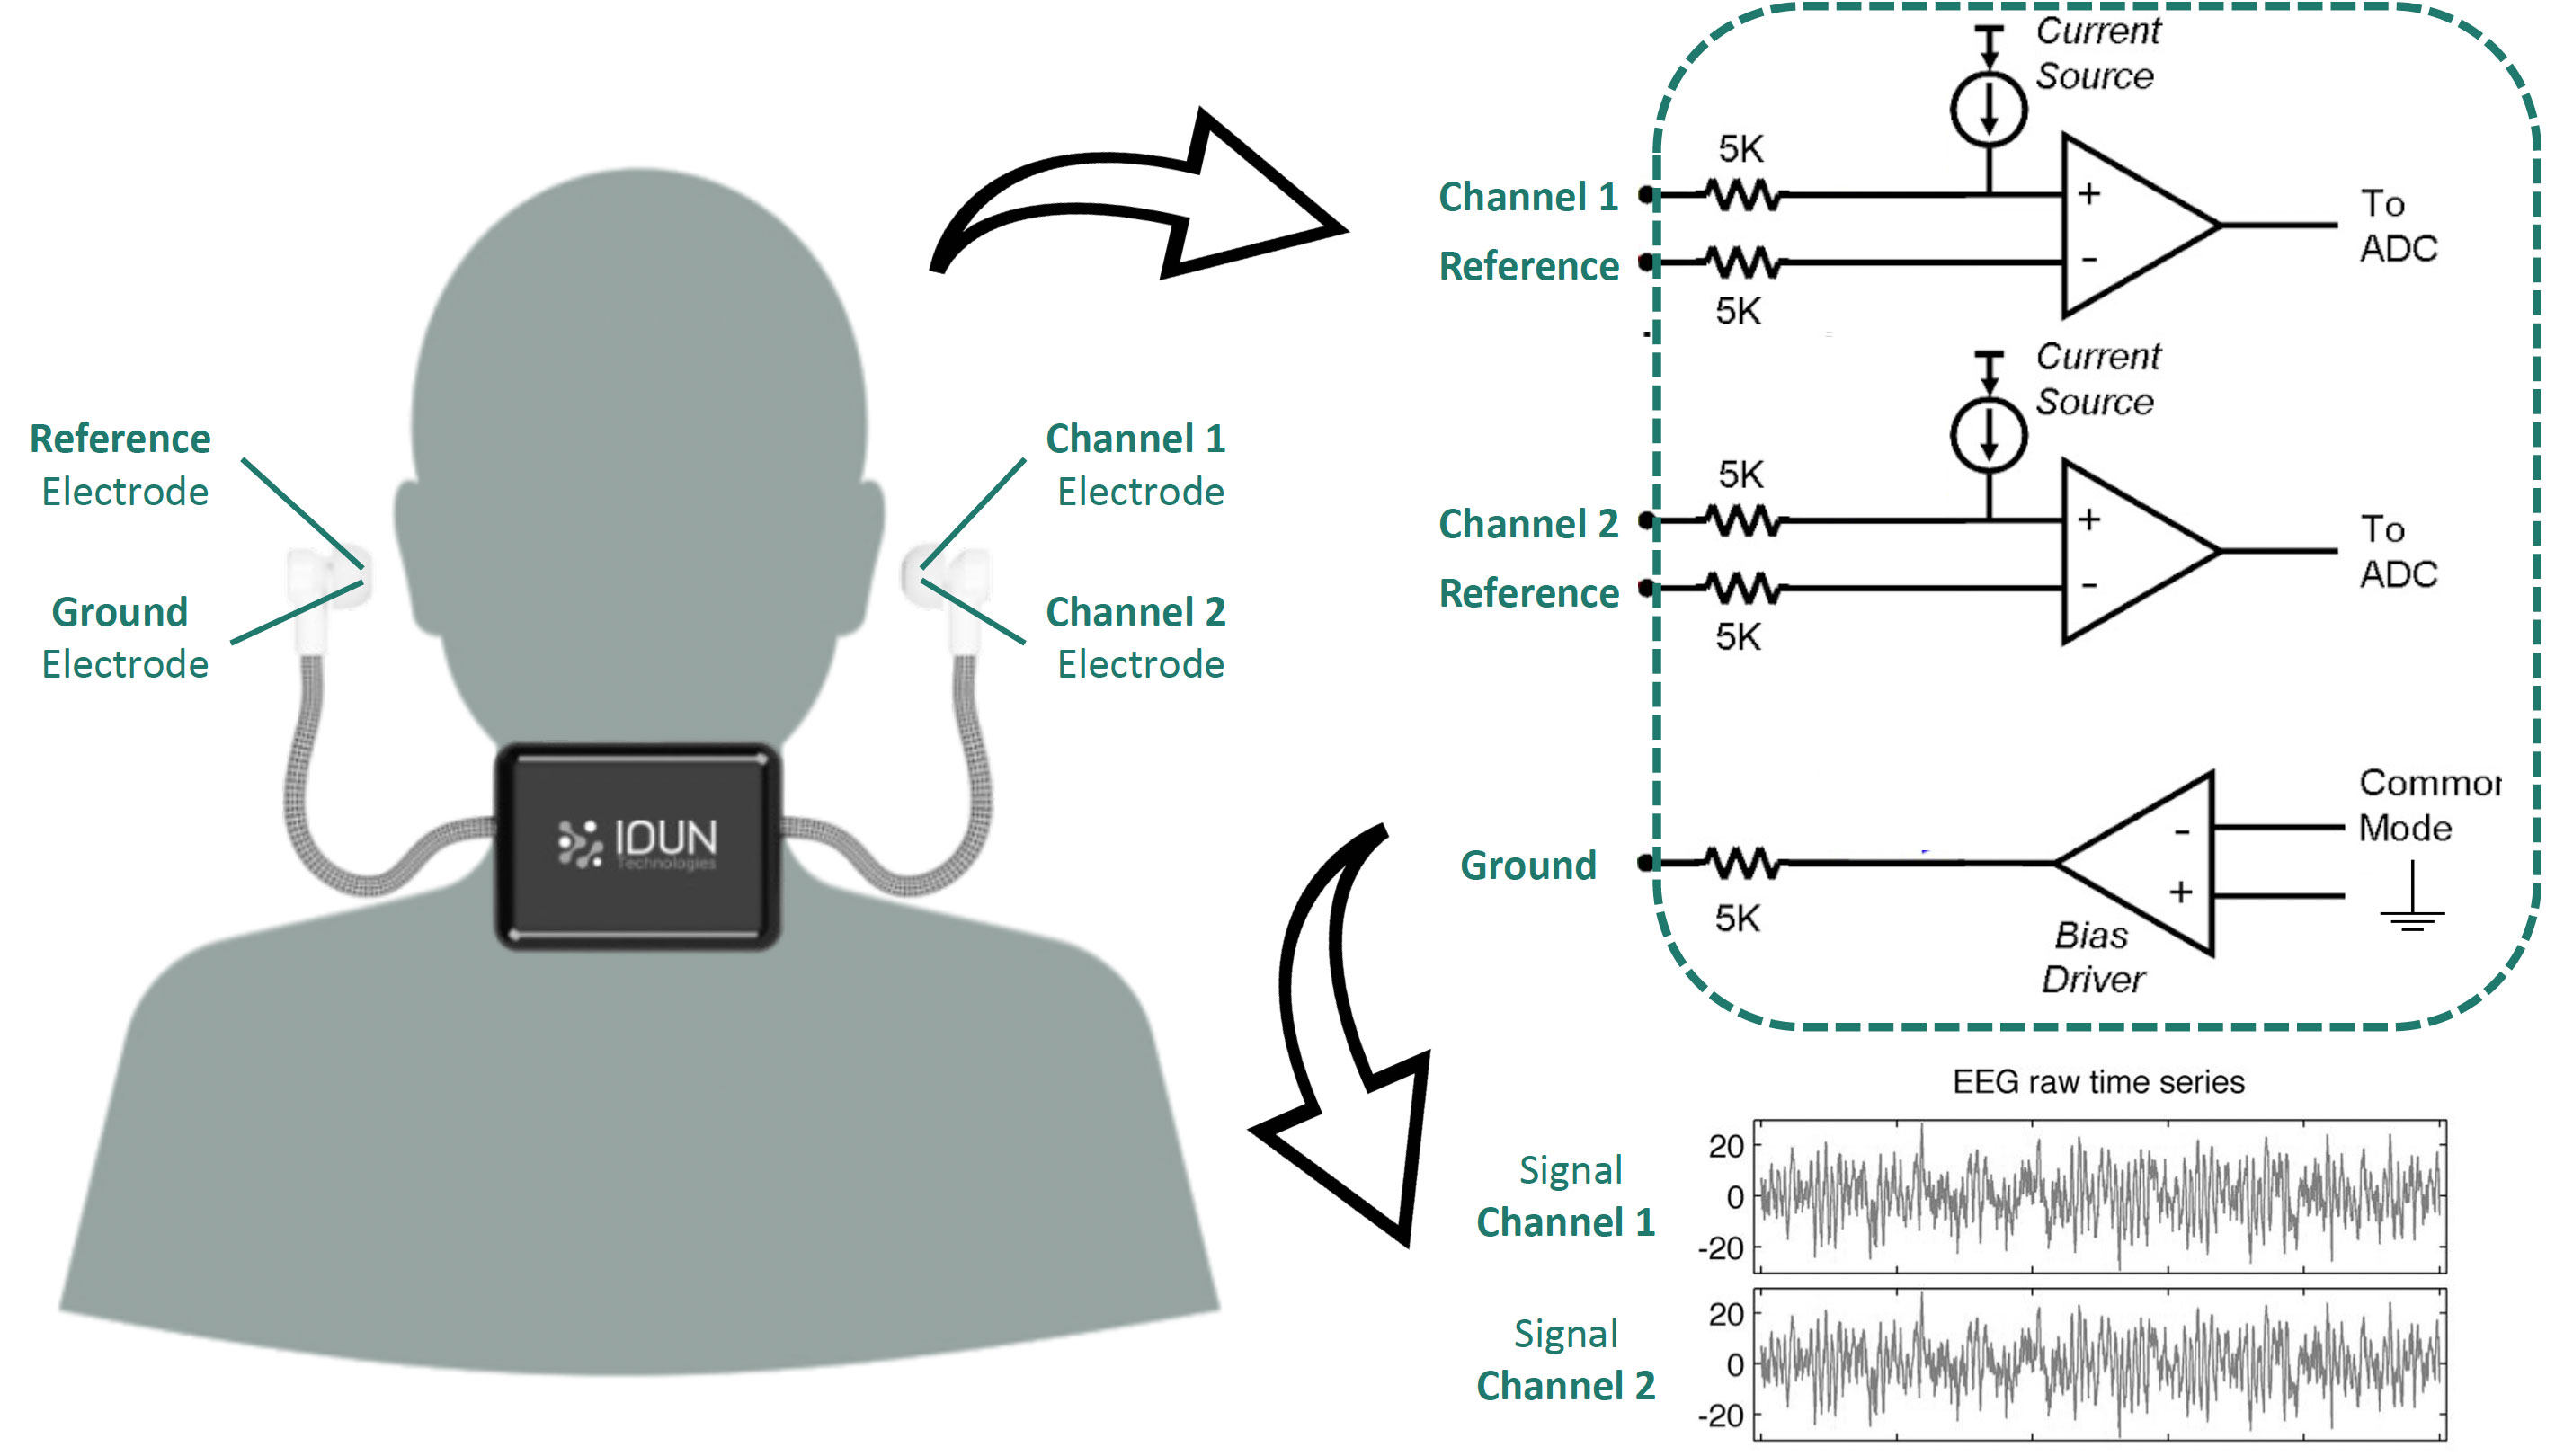
\includegraphics[width=0.75\linewidth]{idun-guardian.jpg}
  \caption{Architecture of the IDUN Guardian hardware (IDUN Technologies, 2022).}
  \label{fig:idun-guardian}
\end{figure}

All these requirements build one of the first mass-market-ready BCI systems, which per definition from the author, form the new concept of a N/CI, which is needed to standardise collaboration and research on this novel sub-discipline of BCI software.

\nomenclature[nlu]{NLU}{Natural language understanding}
\nomenclature[agi]{AGI}{Artificial general intelligence}
\nomenclature[fmri]{fMRI}{Functional magnetic resonance imaging}
\nomenclature[tdfnirs]{TD-fNIRS}{Time-domain functional near-infrared spectroscopy}
\nomenclature[gui]{GUI}{Graphical user interface}
\nomenclature[ssvep]{SSVEP}{Steady-state visual evoked potential}
\nomenclature[ux]{UX}{User experience}
\nomenclature[cli]{CLI}{Command line interface}
\nomenclature[poc]{PoC}{Proof of concept}
\nomenclature[lsl]{LSL}{Lab streaming layer}
\nomenclature[udp]{UDP}{User datagram protocol}
\nomenclature[aws]{AWS}{Amazon Web Services}
\nomenclature[ec2]{EC2}{Elastic Compute Cloud}
\nomenclature[it]{IT}{Information technology}
\nomenclature[vms]{VMs}{Virtual machines}
\nomenclature[gpu]{GPU}{Graphics processing units}
\nomenclature[cpu]{CPU}{Central processing units}
\nomenclature[iot]{IoT}{Internet of Things}
\nomenclature[devops]{DevOps}{Development Operations}
\nomenclature[api]{API}{Application programming interface}
\nomenclature[b2b]{B2B}{Business-to-business}
 % Research Context
%!TEX root = ../thesis.tex

\chapter{My third chapter}
\graphicspath{{Chapter3/Figs/Vector/}{Chapter3/Figs/}}

\section{First section of the third chapter}
And now I begin my third chapter here \dots

\dots and some more 

\subsection{Second subsection in the first section}
\dots and some more \dots

\subsubsection{First subsub section in the second subsection}
\dots and some more in the first subsub section otherwise it all looks the same
doesn't it? well we can add some text to it \dots

\subsection{Third subsection in the first section}
\dots and some more \dots

\subsubsection{First subsub section in the third subsection}
\dots and some more in the first subsub section otherwise it all looks the same
doesn't it? well we can add some text to it and some more and some more and
some more and some more and some more and some more and some more \dots

\subsubsection{Second subsub section in the third subsection}
\dots and some more in the first subsub section otherwise it all looks the same
doesn't it? well we can add some text to it \dots

\section{Second section of the third chapter}
and here I write more \dots

\section{The layout of formal tables}
This section has been modified from ``Publication quality tables in \LaTeX*''
 by Simon Fear.

The layout of a table has been established over centuries of experience and 
should only be altered in extraordinary circumstances. 

When formatting a table, remember two simple guidelines at all times:

\begin{enumerate}
  \item Never, ever use vertical rules (lines).
  \item Never use double rules.
\end{enumerate}

These guidelines may seem extreme but I have
never found a good argument in favour of breaking them. For
example, if you feel that the information in the left half of
a table is so different from that on the right that it needs
to be separated by a vertical line, then you should use two
tables instead. Not everyone follows the second guideline:

There are three further guidelines worth mentioning here as they
are generally not known outside the circle of professional
typesetters and subeditors:

\begin{enumerate}\setcounter{enumi}{2}
  \item Put the units in the column heading (not in the body of
          the table).
  \item Always precede a decimal point by a digit; thus 0.1
      {\em not} just .1.
  \item Do not use `ditto' signs or any other such convention to
      repeat a previous value. In many circumstances a blank
      will serve just as well. If it won't, then repeat the value.
\end{enumerate}

A frequently seen mistake is to use `\textbackslash begin\{center\}' \dots `\textbackslash end\{center\}' inside a figure or table environment. This center environment can cause additional vertical space. If you want to avoid that just use `\textbackslash centering'


\begin{table}
\caption{A badly formatted table}
\centering
\label{table:bad_table}
\begin{tabular}{|l|c|c|c|c|}
\hline 
& \multicolumn{2}{c}{Species I} & \multicolumn{2}{c|}{Species II} \\ 
\hline
Dental measurement  & mean & SD  & mean & SD  \\ \hline 
\hline
I1MD & 6.23 & 0.91 & 5.2  & 0.7  \\
\hline 
I1LL & 7.48 & 0.56 & 8.7  & 0.71 \\
\hline 
I2MD & 3.99 & 0.63 & 4.22 & 0.54 \\
\hline 
I2LL & 6.81 & 0.02 & 6.66 & 0.01 \\
\hline 
CMD & 13.47 & 0.09 & 10.55 & 0.05 \\
\hline 
CBL & 11.88 & 0.05 & 13.11 & 0.04\\ 
\hline 
\end{tabular}
\end{table}

\begin{table}
\caption{A nice looking table}
\centering
\label{table:nice_table}
\begin{tabular}{l c c c c}
\hline 
\multirow{2}{*}{Dental measurement} & \multicolumn{2}{c}{Species I} & \multicolumn{2}{c}{Species II} \\ 
\cline{2-5}
  & mean & SD  & mean & SD  \\ 
\hline
I1MD & 6.23 & 0.91 & 5.2  & 0.7  \\

I1LL & 7.48 & 0.56 & 8.7  & 0.71 \\

I2MD & 3.99 & 0.63 & 4.22 & 0.54 \\

I2LL & 6.81 & 0.02 & 6.66 & 0.01 \\

CMD & 13.47 & 0.09 & 10.55 & 0.05 \\

CBL & 11.88 & 0.05 & 13.11 & 0.04\\ 
\hline 
\end{tabular}
\end{table}


\begin{table}
\caption{Even better looking table using booktabs}
\centering
\label{table:good_table}
\begin{tabular}{l c c c c}
\toprule
\multirow{2}{*}{Dental measurement} & \multicolumn{2}{c}{Species I} & \multicolumn{2}{c}{Species II} \\ 
\cmidrule{2-5}
  & mean & SD  & mean & SD  \\ 
\midrule
I1MD & 6.23 & 0.91 & 5.2  & 0.7  \\

I1LL & 7.48 & 0.56 & 8.7  & 0.71 \\

I2MD & 3.99 & 0.63 & 4.22 & 0.54 \\

I2LL & 6.81 & 0.02 & 6.66 & 0.01 \\

CMD & 13.47 & 0.09 & 10.55 & 0.05 \\

CBL & 11.88 & 0.05 & 13.11 & 0.04\\ 
\bottomrule
\end{tabular}
\end{table}
 % Methodologies
\chapter{Implementation}
% \graphicspath{{Chapter4/Figs/}{Chapter4/Figs/}}

\section{Lorem ipsum}
\label{lorem-ipsum-implementation}

Umfassende und anschauliche (idealerweise Bildmaterial, Screenshots, Zwischenstände. Auch Fehlschläge dokumentieren) Dokumentation was genau getan / erstellt / programmiert / produziert / etc. wurde. Welche Auffälligkeiten gab es? Welche Entscheidungen wurden getroffen? Welche Änderungen / Einschränkungen / Erweiterungen wurden vorgenommen? % Implementation
\chapter{Results and summary}
\graphicspath{{Chapter5/Figs/}{Chapter5/Figs/}}

% 5.1 Ergebnisse: Präsentation des konkreten Endergebnisses. Kompakte Zusammenfassung des Projekts unter Berücksichtigung der anfänglichen Zieldefinition. Wichtig ist dabei, dass man eine kritische Betrachtung der faktischen Resultate vornimmt (Evaluation). Hier ist ein Soll-Ist-Vergleich zur Zielsetzung aus Kapitel 1 mit kritischer Stellungnahme gewünscht. 5.2 Zusammenfassung: Es soll eine Zusammenfassung der Arbeit geschrieben werden und ein Fazit in Bezug auf das Projekt dessen Bedeutung (Relevanz und Nutzen) gezogen werden. Weiterhin soll eine Kritische Betrachtung der eigenen Vorgehensweise erfolgen. Abschließend soll ein Ausblick auf weitere Projektideen, die sich im Rahmen der Arbeit ergeben haben, gegeben werden (Folgeprojekte, Veröffentlichungen, Verwertung). Empfohlener Umfang: ca. 15-20%

\section{Results}
\label{chapter5-results}

\subsection{Key aspects of a N/CI}
\label{chapter5-key-aspects}

\subsubsection{Stream-based events}
\label{chapter5-stream-based-events}
% explain event based architecture and the paradigm-shift in building stream based architectures
% talk about concurrency

\subsubsection{Critical and non-critical}
\label{chapter5-critical-and-non-critical}
% mention the concept from the book and batch processing

\subsubsection{Hardware-accelerated encryption}
\label{chapter5-hardware-accelerated-encryption}
% mention server-side rendering for privacy
% mention discussion with Andy
% TODO show data structure of idun's eeg
% talk about compression and data structure of the EEG data

\subsubsection{Per-device auth and opt-in}
\label{chapter5-user-side-opt-in}
% show opt-in wireframes

\subsubsection{Graph database}
\label{chapter5-graph-database}
% explain MLOps and outlook with Kubeflow
% mention data lakes and data warehouse
% mention internal SDK for feature extraction and experiments
% what is feature extraction and the process
% show image from Wadda

% However, in practice, it appears that simply making data available quickly—even if it is in a quirky, difficult-to-use, raw format—is often more valuable than trying to decide on the ideal data model up front [54].

\subsection{Example architecture of a N/CI}
\label{chapter5-example-architecture-of-a-nci}

% split by key components
% show what i've drawn on the whiteboard at work for event-driven architecture

% Performance
% Scalability
% Reliability
% Security
% Deployment
% Technology Stack

% TODO show entire architecture chart and split into sections and go through them figure by figure

% - First, we investigated whether X (research question)
% - We used an Independent samples t test with groups as independent variable and the
% depression score as dependent variable
% - The results showed that the difference between the groups/ conditions was significant
% - The results showed a significant correlation between…
% - The results showed a significant interaction between…
% - Specifically, the average depressions score was lower in the treatment group (M=3.45, SD = 2.18) compared to the placebo group (M=4.83, SD = 2.02).

% Always show measure of success per each part of the architecture (say that going into detail of performance indicators and security is not part of this thesis)
% talk about achieved goals

% o Did you describe everything that is needed to replicate your results?
% o Did you describe all pre-processing steps before the main analyses?
% o Did you mention to which research question each analysis belongs?
% o Did you avoid interpreting your results?
% o Did you add figures for making your key results easy to understand (or are they very simple)?
% o Did you add tables for extensive amounts of (numerical) information?

% o Does your discussion go from specific (interpretation) to broad (implications)?
% o Did you draw conclusions with reservations? (“A possible interpretation is…”)
% o If you expressed a preference for one explanation over another, did provide clear
% support for this preference?
% o Did you describe how your research connects to previous research?
% o Did you make clear what your research adds to existing research?
% o Did you describe how your research advance our understanding or how they may inspire
% future applications?
% o Did you clearly admit limitations before qualifying them?
% o Did you remind the reader of the value/implications of your research at the end?
% o Did you include some pointers for future research? (optional)

% non-trivial, n-body system, Services, batch processing and near real time streaming, shared nothing, encrypted, total order broadcast etc. => all insights that were gained for the N/CI and the task to define a N/CI on its own as well + Systems of record and derived data system (p 602 to cite) ==> add some parts to the implementation chapter

\section{Summary}
\label{chapter5-summary}

\subsection{Reflection}
\label{chapter5-reflection}

\subsection{Outlook}
\label{chapter5-outlook}
% mention to publish the thesis somewhere if possible with the help of IDUN
% further development into deep learning models and more detailed description of a N/CI on the cloud rather then "just" introducing and displaying the most important aspects and components => could be done in a MSc

\subsection{Conclusion}
\label{chapter5-conclusion}

% - We investigated whether depression can be treated by training a positive focus
% - Our findings confirm this
% - Novel perspective on depression
% - More research needed, more treatments that follow this approach should be developed
 % Results and Summary

% Passing the `heading` argument to include the bibliography in the TOC
\printbibliography[heading=bibintoc]

\begin{appendices}
  \chapter{Definition and motivation of a N/CI}
\label{appendix1-definition-and-motivation-of-a-nci}
\graphicspath{{Appendix1/Figs/}{Appendix1/Figs/}}

This section discusses the definition, need and differentiation of a N/CI and the paradigm shifts associated with it when discussing BCI software.

\section*{BCI software on the cloud}
\label{appendix1-bci-software-on-the-cloud}

Looking at \autoref{fig:nci-components}, we can see that the three software layers of a BCI-component illustration, as pictured on \autoref{fig:bci-components} are highlighted. This is due to the fact that these components are not bound to a physical interface such as a cable or Bluetooth.

\begin{figure}[ht]
  \centering
  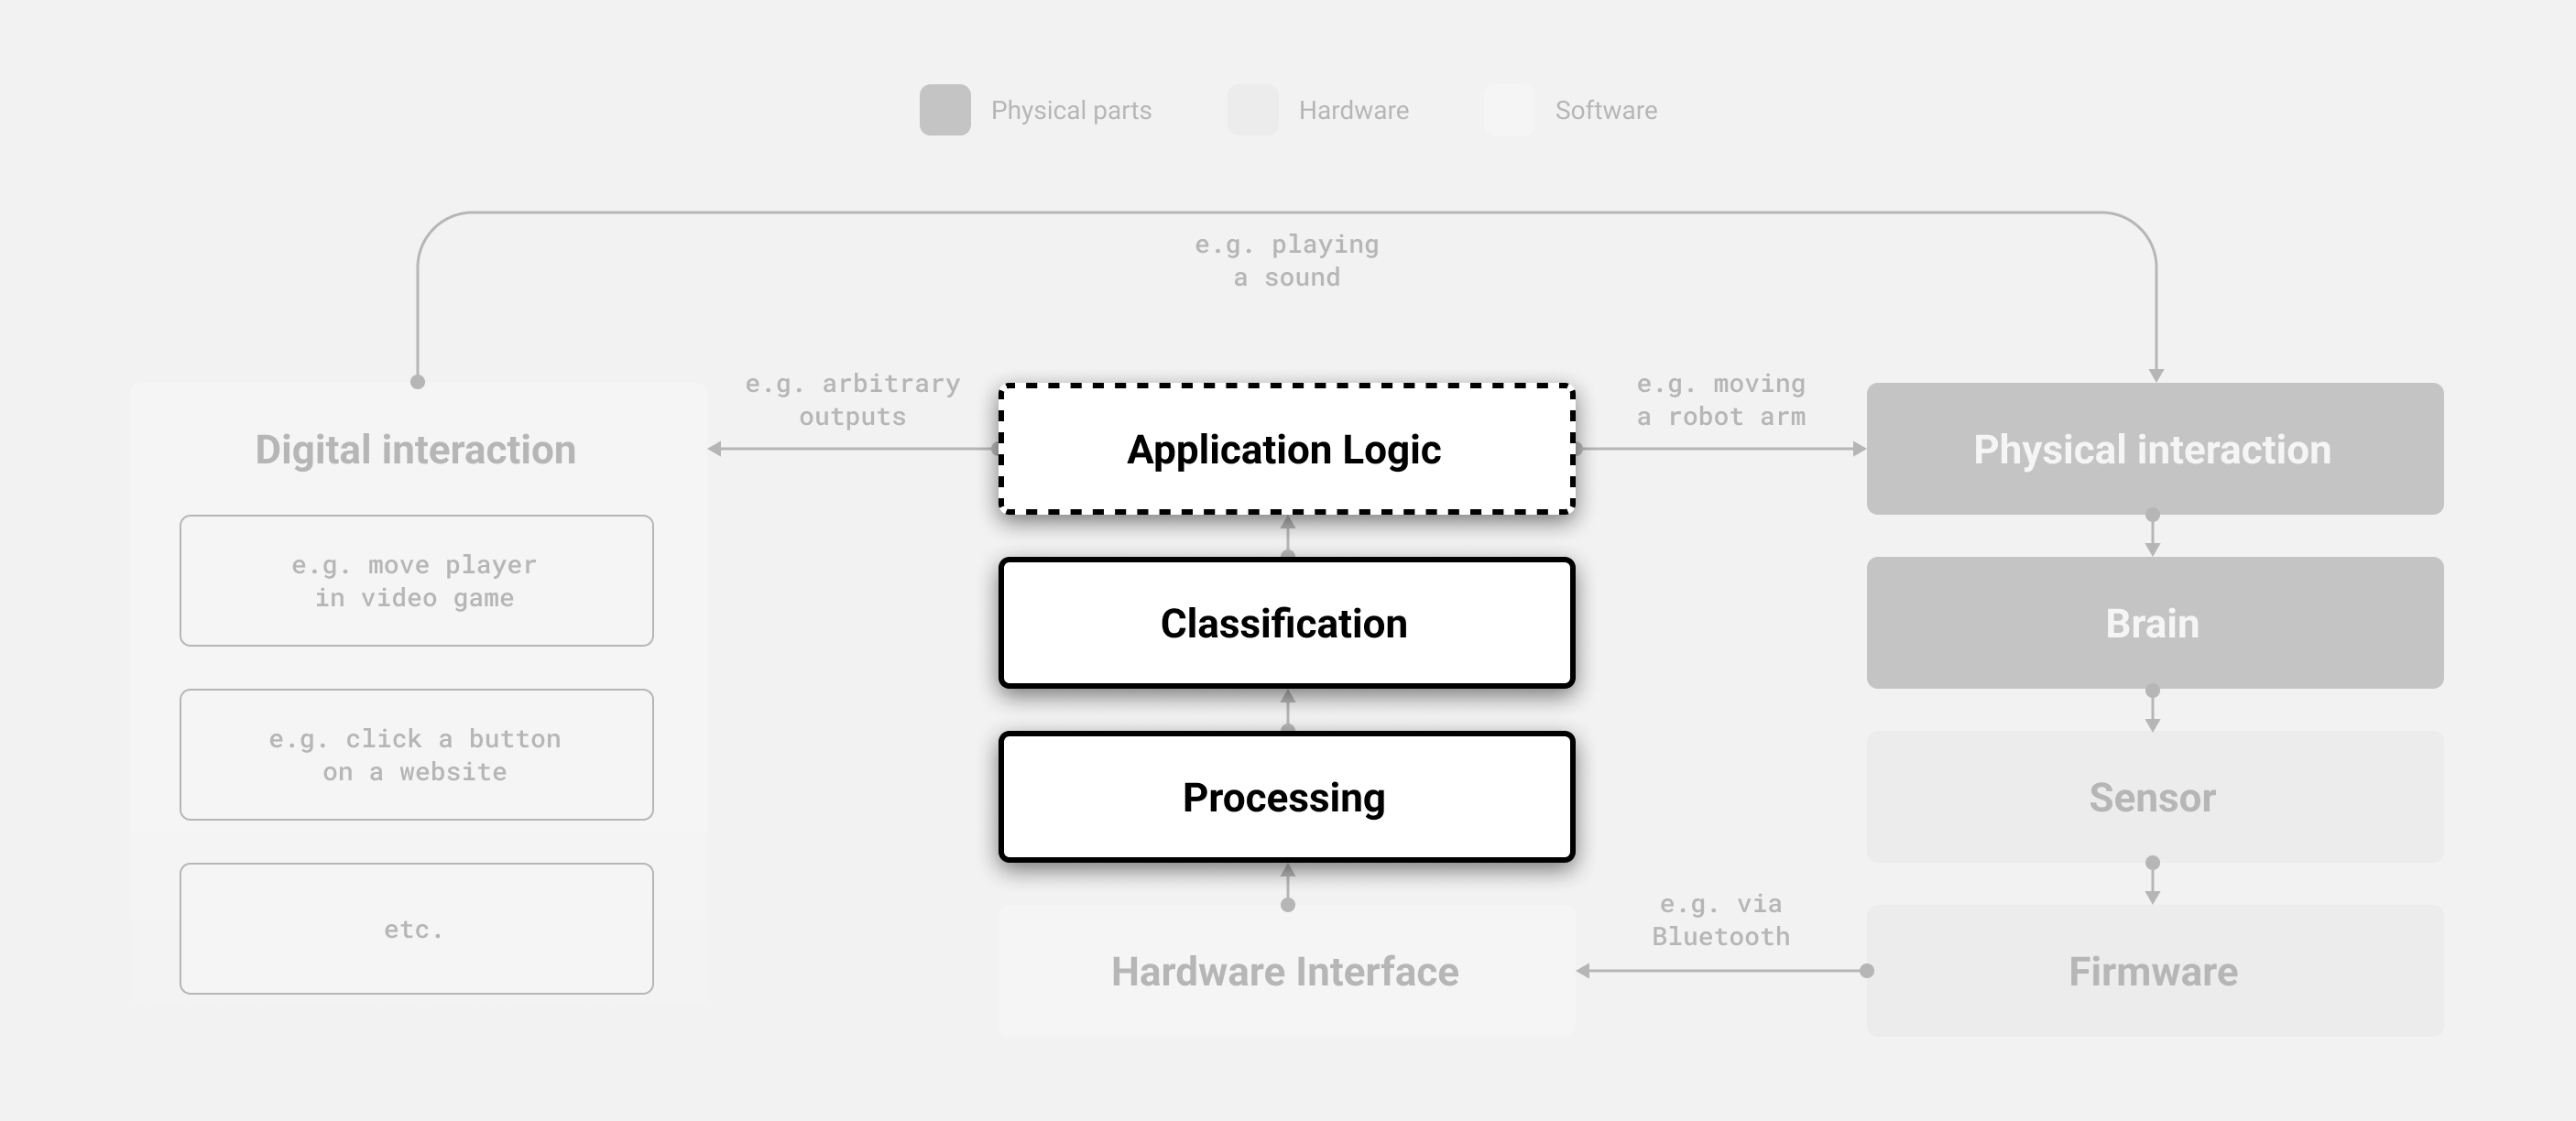
\includegraphics[width=\linewidth]{nci-components.png}
  \caption{Highlighted software components as previously shown on \autoref{fig:bci-components} of a BCI that could be moved to the cloud.}
  \label{fig:nci-components}
\end{figure}

Running software on the cloud means that developers or companies can access provisioned information technology (IT) infrastructure through the internet, usually with a pay-as-you-go pricing model \citep{amazon_web_services_inc_what_nodate}. The development speed of software applications can drastically improve since software developers can only focus on software rather than incorporating the hardware and network aspect of setting up their server farms, therefore abstracting the hardware part away. What started with simple computers that can be rented in a remote server farm such as it was with, e.g. Amazon Web Services (AWS) Elastic Compute Cloud (EC2) \citep{barr_amazon_2006} ended up being a diverse offering from cloud providers with various abstraction levels as shown in \autoref{tab:cloud-computing-types}.

\begin{table}[!ht]
  \centering
  \resizebox{\textwidth}{!}{%
    \begin{tabular}{ll}
      \rowcolor[HTML]{000000}
      {\color[HTML]{FFFFFF} Type}                                                                                 &
      {\color[HTML]{FFFFFF} Description}                                                                                                                                                                                                                                                                                                                           \\ \hline
      \multicolumn{1}{|l|}{\textbf{\begin{tabular}[c]{@{}l@{}}Infrastructure as\\ a Service (laaS)\end{tabular}}} &
      \multicolumn{1}{l|}{\begin{tabular}[c]{@{}l@{}}IaaS gives access to data storage space, virtual or dedicated\\ computers, and network services. The greatest degree of\\ flexibility and administrative control over your IT resources\\ are provided by utilising IaaS.\end{tabular}}                                                                       \\ \hline
      \multicolumn{1}{|l|}{\textbf{\begin{tabular}[c]{@{}l@{}}Platform as a\\ Service (PaaS)\end{tabular}}}       &
      \multicolumn{1}{l|}{\begin{tabular}[c]{@{}l@{}}PaaS lets developers concentrate on developing and\\ managing their code rather than worrying about the\\ underlying infrastructure (often hardware and operating\\ systems). An example is Kubernetes.\end{tabular}}                                                                                         \\ \hline
      \multicolumn{1}{|l|}{\textbf{\begin{tabular}[c]{@{}l@{}}Software as a\\ Service (SaaS)\end{tabular}}}       &
      \multicolumn{1}{l|}{\begin{tabular}[c]{@{}l@{}}SaaS provides a whole product that is run and controlled \\ by the service provider. The phrase SaaS often refers to\\ end-user apps (e.g. web-based email). Developers don't\\ have to be concerned about how the service is handled\\ or whether the underlying infrastructure is maintained.\end{tabular}} \\ \hline
    \end{tabular}%
  }
  \vspace{10pt}
  \caption[The three abstraction levels and types of cloud computing]{The three abstraction levels and types of cloud computing \citep{amazon_web_services_inc_what_nodate}.}
  \vspace{-5pt}
  \label{tab:cloud-computing-types}
\end{table}

The majority of businesses are anticipated to embrace a cloud-first strategy by 2025, according to Milind Govekar, vice president of IT research and consultancy company Gartner, and will not be able to fully implement their digital plans without the usage of cloud-native architectures and technologies \citep{gartner_gartner_nodate}. The impact and importance of cloud computing cannot be underestimated, and its success is also reflected in the annual spending on cloud computing resources, estimated at €474 billion in 2022 \citep{gartner_gartner_nodate}. Cloud computing is such an extensive and complex topic that it could quickly fill entire books. The author categorises three broad but essential points that certainly play a vital role in BCI software: 1. Dedicated and deterministic environments, which explains that an environment of a software programme always stays the same independent of the end-users hardware, 2. elastic and high-performance availability, which explains cloud computers that have an on-demand and adjustable high-performance and 3. provided services for speed, which explains the concept of pre-made and dedicated software written primarily for the cloud and specific use cases. The following list goes more into detail about the mentioned topics in the context of BCI software:

\begin{enumerate}
  \item \textbf{Dedicated and deterministic environments:} Running code for BCIs on different end-user platforms, such as Windows or Android, can have drawbacks because each device has its processor, graphics card, operating system version and drivers, which can make developing software that requires stable and good performance, such as neural data processing pipelines, time-consuming and difficult to maintain, as developers must keep track of every factor of the end-user devices. This is fine for BCIs that are not intended for the general public, such as specially designed BCIs for people with, say, locked-in syndrome, but for the general public, a vast amount of different end-user devices could come into play. When code runs on a dedicated machine, such as a cloud computer with clearly defined hardware and operating system specifications, it becomes less error-prone and more deterministic.
  \item \textbf{Elastic and high-performance availability:} Because the cloud usually runs as an as-needed model, the initial purchase cost of computer hardware is split and shared across usage. Developers have access to tremendous computing power that would not be easily afforded if purchased independently. As a result, when developing a computationally intensive algorithm, developers can use high-performance central processing units (CPUs) and graphics processing units (GPUs) to complete tasks much faster than consumer hardware on end-user devices. Performance can also be increased as needed, e.g. to handle computationally heavier tasks that are not used as frequently or to handle more requests when, e.g. the demand for the software increases due to an increase in the number of users, which is a process known as elasticity \citep{gartner_definition_nodate}. Furthermore, the cloud provides far more storage capacity than end-user devices.

  \item \textbf{Provided services for speed:} The vast majority of cloud providers are providing more specialised services as we move closer to PaaS. Provisioned database servers, for example, exist solely to serve as a database, so the underlying hardware is optimised for the database software running on it. Hundreds of cloud computing services are available, including 200 from AWS alone \citep{amazon_web_services_inc_what_nodate}, all of which address specific use cases. This is extremely useful when it comes to cloud-based BCI software. One example is the aspect of live streaming of brain data, which we will go over in greater detail in the implementation chapter of this thesis. The services accelerate development speed by eliminating the need for teams to reinvent the wheel repeatedly, next to also providing out-of-the-box scalability due to built-in elasticity and the concept of fully abstracted hardware via the serverless model  \citep{redhat_what_2022}.
\end{enumerate}

A N/CI utilises cloud computing by running certain software components of a BCI system in the cloud with the benefits as mentioned before. Multiple BCIs can communicate with each other or with other software or hardware over the internet, enabling remote human-computer interaction. \autoref{fig:nci-overview} depicts how two or more BCIs can interface with one another using cloud software. The red arrows represent the typical local BCI. The blue arrow depicts how BCI B  can execute business logic via the cloud over the internet, enabling digital and physical interactions with, e.g. high performance. The green arrow depicts how BCI A can communicate via a N/CI with BCI B even if they are not in the same geographical location.

\begin{figure}[ht]
  \centering
  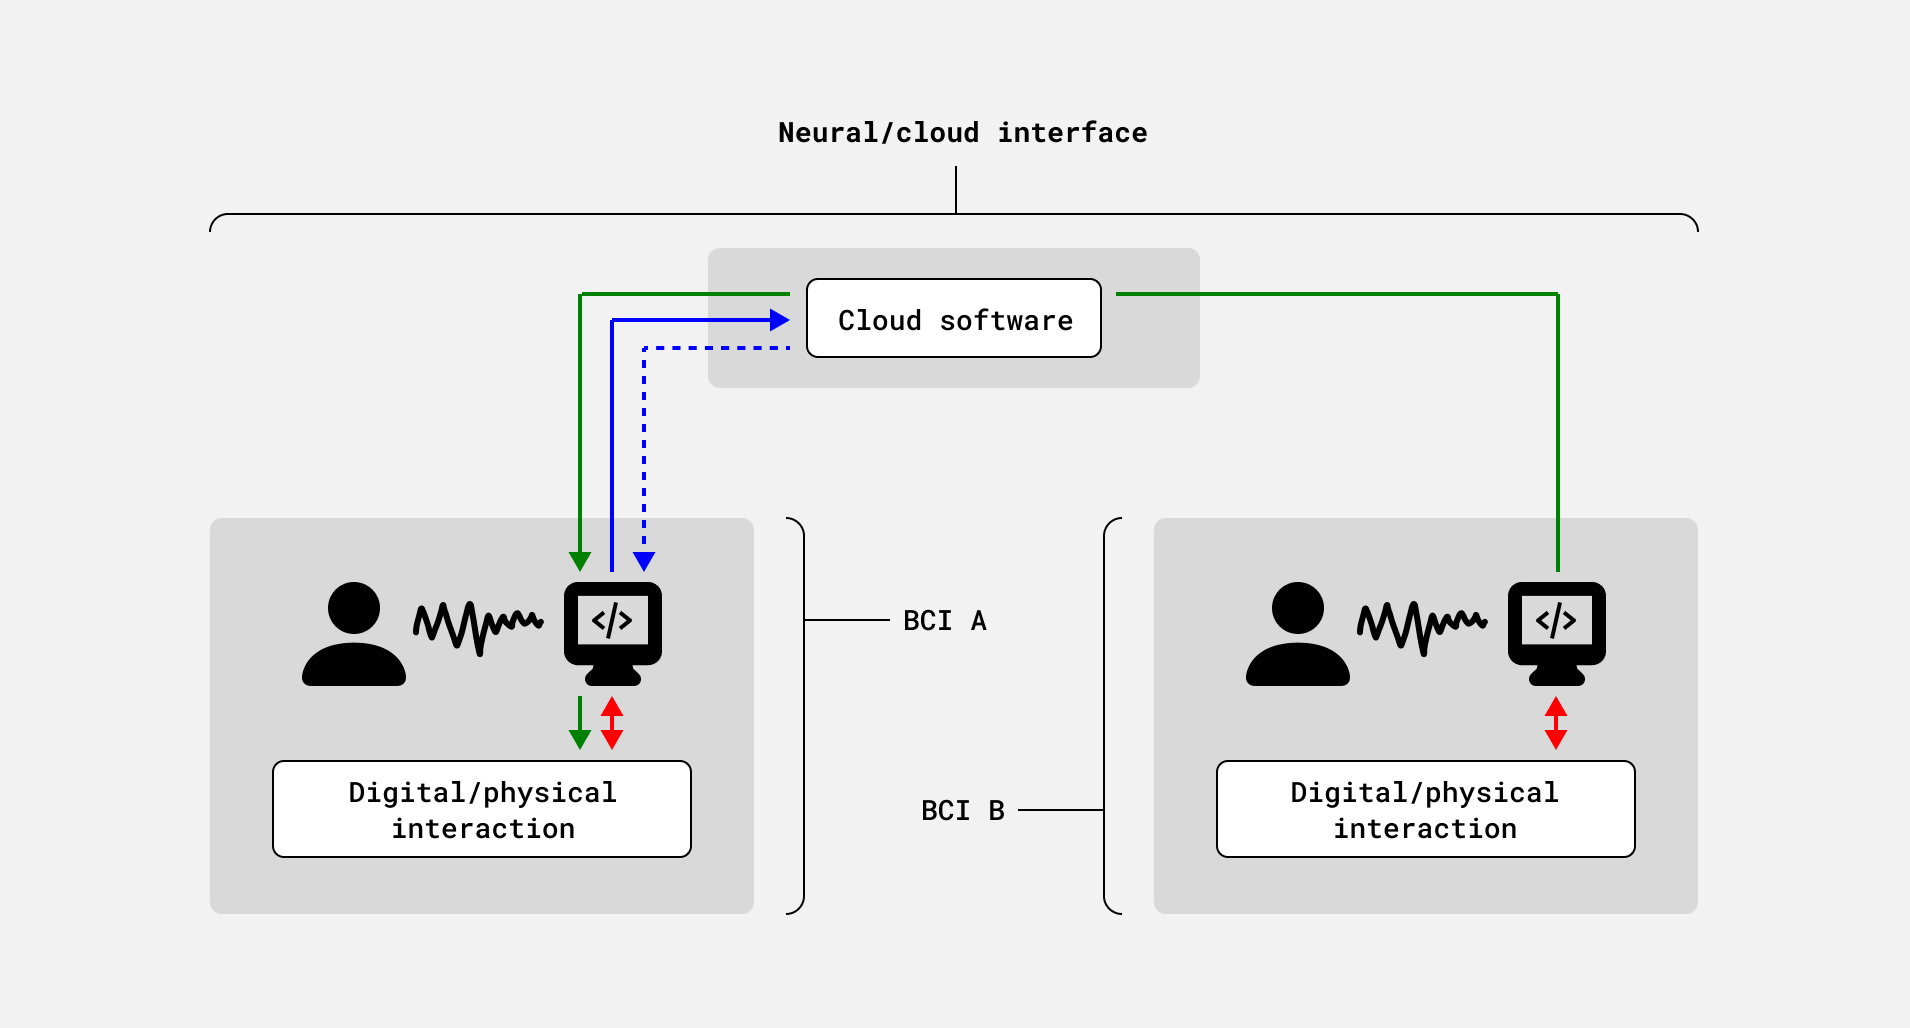
\includegraphics[width=\linewidth]{nci-overview.png}
  \caption{A N/CI is the connection between multiple BCIs.}
  \label{fig:nci-overview}
\end{figure}

\section*{Distinction between existing research}
\label{appendix1-distinction-between-existing-research}

The concept of running BCI software components remotely and on the cloud is not novel, as research into the concept known as asynchronous BCI \citep{an_design_2016} or internet-based BCI \citep{lampe_brain-computer_2014} has been ongoing for some time. However, when we look at the more recent research from \citeauthor{zhang_internet_2018} on their cloud-based deep learning framework to enable, as they describe Human-Thing Cognitive Interactivity, we see a strong emphasis on algorithms and machine learning but less on aspects such as the cloud architecture and mass-market-readiness \citep{zhang_internet_2018}. They address the latency and the size of EEG samples sent in near-real-time to a server, as well as the corresponding calculation, but there are no more details in regards to the proposed and very simplified architecture chart's components or effective cloud architecture, all of which factor into the author's aim to develop a N/CI. Another related and even more recent paper by \citeauthor{ahamad_system_2022} looks at the system architecture of a BCI for the Internet of Things (IoT), but this time from the perspective of algorithms optimised for time series data such as EEG, but still with no mention of the effective cloud architecture of such a system \citep{ahamad_system_2022}.

The author of this thesis introduces the concept of three-dimensionality for the definition of a N/CI based on the previously mentioned topics and research that touch on the issues of this thesis, which are essential to achieve general applicability for BCIs from the perspective of the software system for the actual implementation of such a system.

\section*{Requirements of a N/CI}
\label{appendix1-requirements-of-a-nci}

The term N/CI positions itself as a software system in the intersection that can undoubtedly be defined as production-grade rather than being in the PoC stage, unobtrusive implementation rather than obtrusive software and general-purpose applicability rather than being made just for a specific use case. \autoref{fig:nci-definition} illustrates the position of a N/CI within the mentioned properties. Subsequently, \autoref{tab:nci-axis} summarises the definitions as described in this thesis.

\captionsetup[figure]{list=no}

\begin{figure}[ht]
  \centering
  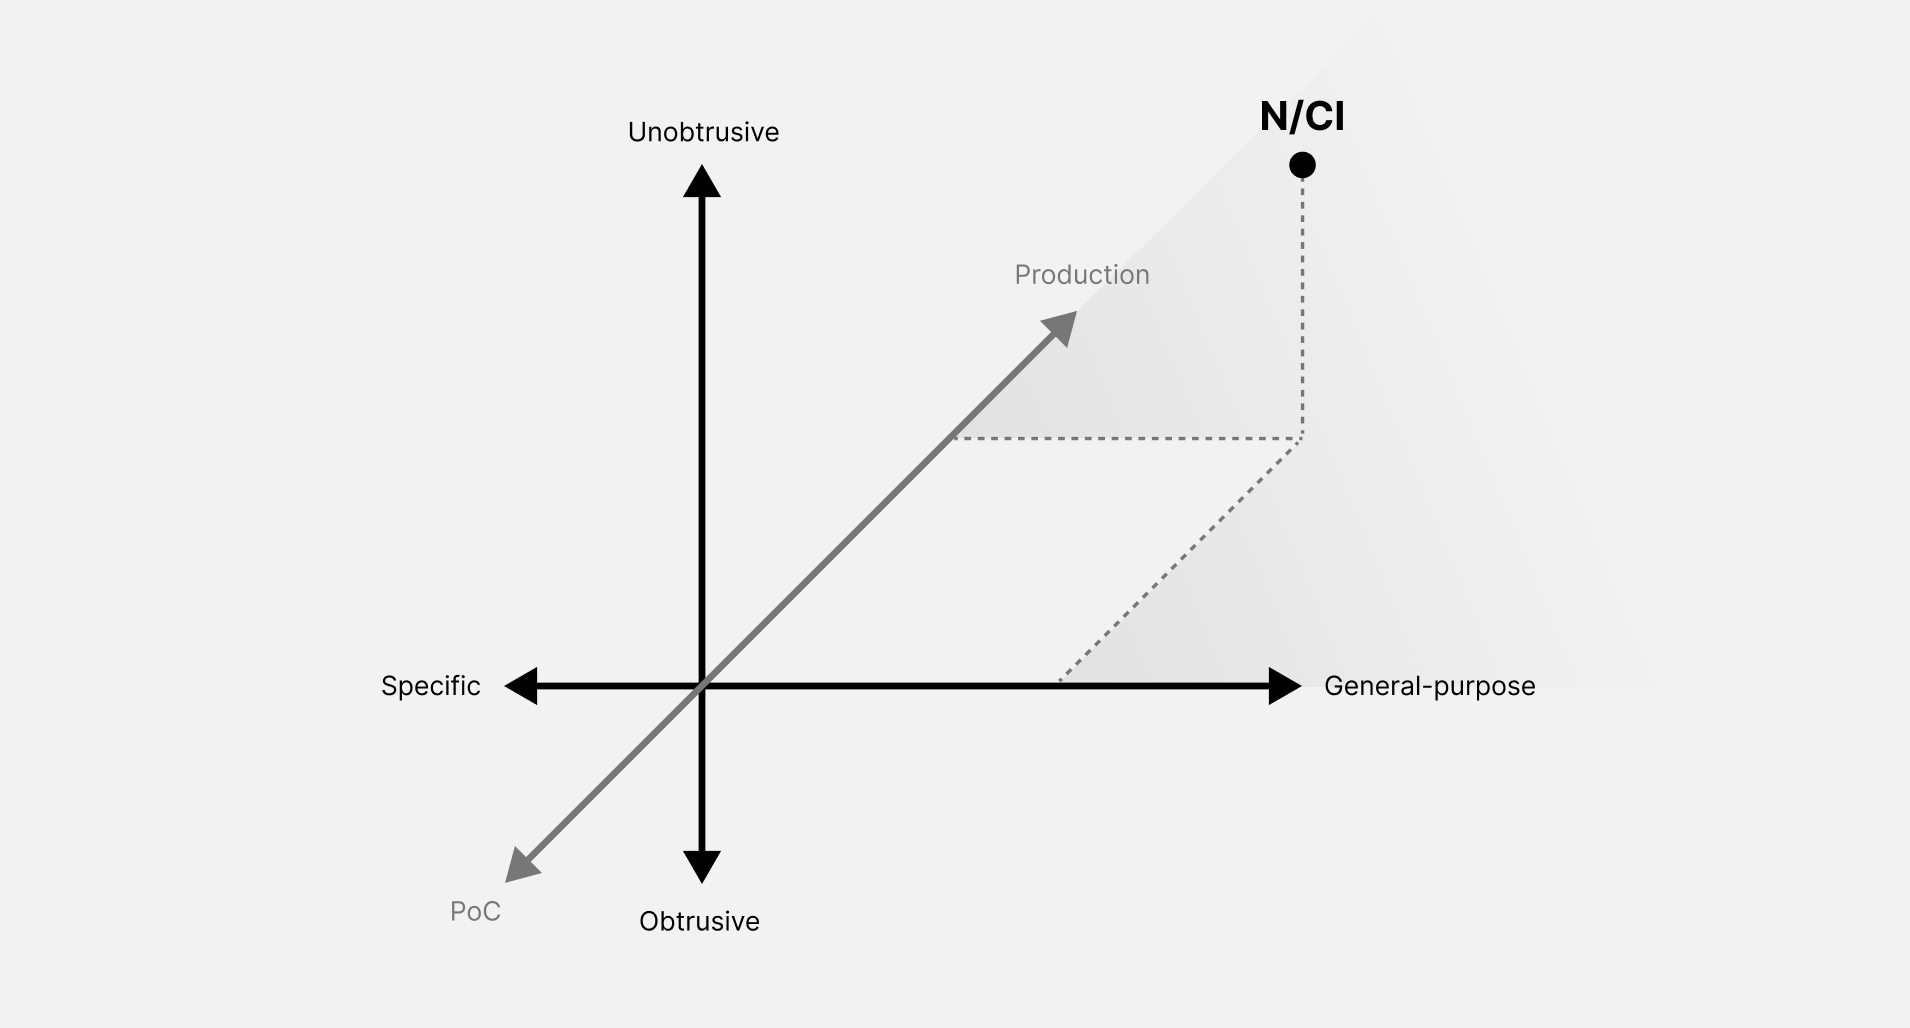
\includegraphics[width=\linewidth]{nci-definition.png}
  \caption{Visualisation of the three-dimensionality of the term neural/cloud interface with its three axes and differentiation of six terms.}
  \label{fig:nci-definition}
\end{figure}

\captionsetup[figure]{list=yes}


\begin{table}[ht]
  \centering
  \resizebox{\textwidth}{!}{%
    \begin{tabular}{ll}
      \rowcolor[HTML]{000000}
      {\color[HTML]{FFFFFF} Axis labelling}                   &
      {\color[HTML]{FFFFFF} Description}                                                                                                                                                                                                                                                                                                                                                                                                                                                                                                                                                                                  \\ \hline
      \multicolumn{1}{|l|}{\textbf{Production}}               &
      \multicolumn{1}{l|}{\begin{tabular}[c]{@{}l@{}}As previously stated, this is the range in which a software system is deemed ready for production.\\ Because the definition is vague, it is difficult to identify specific requirements that must be met for\\ a system to be considered production-ready. However, for a N/CI, this means running in a\\ production environment, e.g. in a cloud, on a real-world end-user server rather than, for example,\\ in a proof-of-concept environment such as in a lab.\end{tabular}}                                                                                     \\ \hline
      \multicolumn{1}{|l|}{\textbf{Unobtrusive}}              &
      \multicolumn{1}{l|}{\begin{tabular}[c]{@{}l@{}}As previously stated, an unobtrusive software system is one in which the end-user does not need\\ to understand the underlying architecture and requirements in order to use the software or even\\ know certain parts of the software system. In the reverse case, users need to install special\\ packages or download additional companion apps to make a N/CI work on their computer\\ or smartphone is not the aim of the author's definition of a N/CI.\end{tabular}}                                                                                          \\ \hline
      \multicolumn{1}{|l|}{\textbf{General-purpose}}          &
      \multicolumn{1}{l|}{\begin{tabular}[c]{@{}l@{}}A general-purpose software system is one that can be used for a variety of functions. As an\\ example, consider AWS. It is general-purpose, which means that developers can create\\ cloud software on AWS that can be either a financial application or a backend for a mobile\\ game; there are no specific use cases. This means that a N/CI, unlike the NextMind BCI\\ or the Muse headband, should provide general-purpose functionality rather than specific use\\ cases, i.e. it is not limited to a specific set of functions.\end{tabular}}                 \\ \hline
      \rowcolor[HTML]{EFEFEF}
      \multicolumn{1}{|l|}{\cellcolor[HTML]{EFEFEF}PoC}       &
      \multicolumn{1}{l|}{\cellcolor[HTML]{EFEFEF}\begin{tabular}[c]{@{}l@{}}A BCI software system that serves as a proof of concept cannot be considered N/CI because\\ it is not intended for production and thus all the effort required to create a production system,\\ such as quality assurance with unit or end-to-end testing, is unnecessary. A PoC system does\\ not usually run in a production environment, as the goal is, for example, to test a specific\\ functionality of a use case rather than to deliver the software to end-users.\end{tabular}}                                                    \\ \hline
      \rowcolor[HTML]{EFEFEF}
      \multicolumn{1}{|l|}{\cellcolor[HTML]{EFEFEF}Obtrusive} &
      \multicolumn{1}{l|}{\cellcolor[HTML]{EFEFEF}\begin{tabular}[c]{@{}l@{}}An obtrusive BCI system, for example, may still be production-ready if it targets specific use cases\\ while remaining unobtrusive because neuroscientists or developers, for example, expect to have\\ access to the underlying software architecture or technical requirements and thus do not want to\\ abstract from it. If it is obtrusive software, such as OpenBCI, this usually means building the\\ production-ready part on top of it is necessary, which does not fit the author's proposed definition\\ of a N/CI.\end{tabular}} \\ \hline
      \rowcolor[HTML]{EFEFEF}
      \multicolumn{1}{|l|}{\cellcolor[HTML]{EFEFEF}Specific}  &
      \multicolumn{1}{l|}{\cellcolor[HTML]{EFEFEF}\begin{tabular}[c]{@{}l@{}}If a BCI system is only used for one use case, such as Muse for sleep and meditation, companies\\ or developers who want to offer a different use case, such as a mind-controlled keyboard with a\\ P300 system will have to reverse engineer Muse's EEG output or use a different BCI hardware\\ that is less specific and closed, and then build their own production-ready and unobtrusive software\\ on top of it.\end{tabular}}                                                                                                         \\ \hline
    \end{tabular}%
  }
  \vspace{10pt}
  \caption{Axes label descriptions of the three-dimensionality for the definition of a N/CI as shown on \autoref{fig:nci-definition}.}
  \label{tab:nci-axis}
\end{table}

\newpage

With an unobtrusive form factor like the one developed by IDUN Technologies, a significant hardware barrier to becoming a mass-market BCI has already been tackled. Next to the hardware, IDUN intends to provide a business-to-business (B2B) software platform, allowing 3rd-party developers to create software on top of IDUN's offerings through a universal brain application programming interface (API). Because they allow others to consume this API in end-user-facing apps, it must be production-ready and unobtrusively able to be integrated. IDUN's hardware and software aim to be general-purpose rather than specific, allowing others to build any BCI-enhanced app \citep{idun_guardian_nodate}.

All of IDUN's requirements systematise one of the first BCI aimed at the general public, which satisfies the broad definition of a N/CI. The fundamental motivation of the author is to standardise collaboration and research on this novel and interdisciplinary field of BCI software and cloud computing.

  \chapter{Group discussion notes}
\label{appendix2-group-discussion-notes}

\section*{Important notes: First kick-off meeting}

\section*{Important notes: Mid-way collaboration meeting}

\section*{Important notes: Closing meeting}

  \chapter{User interviews and outline}
\label{appendix3-user-interviews-and-outline}

This appendix chapter lists the outline and rough framework used to conduct the user interviews, as well as the notes taken by the author and IDUN’s product manager, Mark Melnykowycz, during the interview sessions. The notes are represented in the state they were in at the time of recording. The focus was on conducting user interviews especially in the Robbie and Evan personas, as they were the first actual users of the software platform targeted by the C-level management.

\section*{User interview outline for the Robbie persona}

Notion PDF export to be found in the file \textit{user\_interview\_with\_a\_robbie.pdf} in the appendices directory in the user interviews subdirectory.

\section*{User interview outline for the Evan persona}

Notion PDF export to be found in the file \textit{user\_interview\_with\_an\_evan.pdf} in the appendices directory in the user interviews subdirectory.

\section*{User interview with Paul Doyle}

Notion PDF export to be found in the file \textit{user\_interview\_with\_paul.pdf} in the appendices directory in the user interviews subdirectory.

\section*{User interview with Ghena Hammour}

Notion PDF export to be found in the file \textit{user\_interview\_with\_ghena.pdf} in the appendices directory in the user interviews subdirectory.

\section*{User interview with Nicole Zahnd}

Notion PDF export to be found in the file \textit{user\_interview\_with\_nicole.pdf} in the appendices directory in the user interviews subdirectory.

\section*{User interview with Melanie Baumgartner}

Notion PDF export to be found in the file \textit{user\_interview\_with\_melanie.pdf} in the appendices directory in the user interviews subdirectory.

\section*{User interview with Mayank Jain}

Notion PDF export to be found in the file \textit{user\_interview\_with\_mayank.pdf} in the appendices directory in the user interviews subdirectory.

\section*{User interview with Martin Hutchings}

Notion PDF export to be found in the file \textit{user\_interview\_with\_martin.pdf} in the appendices directory in the user interviews subdirectory.

\section*{User interview with Jacopo de Araujo}

Notion PDF export to be found in the file \textit{user\_interview\_with\_jacopo.pdf} in the appendices directory in the user interviews subdirectory.

\section*{User interview with Garrett Flynn}

Notion PDF export to be found in the file \textit{user\_interview\_with\_garrett.pdf} in the appendices directory in the user interviews subdirectory.


  \chapter{Web-first approach proposal}
\label{appendix4-web-first-approach-proposal}

  \chapter{Design artefacts}
\label{appendix5-design-artefacts}

\section*{First console web app wireframes}

\section*{Second console web app wireframes}

\section*{Auth page wireframes}

\section*{User journey architecture}

\end{appendices}
\end{document}
